\section{Simulating RNA-seq library construction using \rlsim}

\subsection{Quick reference}
\label{ss:qrlsim}

\begin{verbatim}
Simulate RNA-seq library preparation with priming biases, PCR biases and size selection 
(version: 1.0).

Usage:
        rlsim [arguments] [transcriptome fasta files (optional)]

Optional arguments:
                argument                    type    default  
        -n      requested fragments         int     
        -d      fragment size distribution  string  [check source]
        -f      fragmentation method        string  "after_prim_double"
        -b      strand bias                 float   0.5
        -c      PCR cycles                  int     11
        -p      priming bias parameter      float   5.0
        -k      primer length               int     6
        -a      poly(A) tail size dist.     string  [check source]
        -flg    fragment loss probability   float   0.0
        -m      expression level multiplier float   1.0
        -e      fixed PCR efficiency        float   0.0
        -eg     GC efficiency parameters 
                as "(shape, min, max)":
                    shape                   float   8.0
                    min                     float   0.8
                    max                     float   0.95
        -el     length efficiency parameters 
                as "(shape, min, max)":
                    shape                   float   0.0
                    min                     float   1.0
                    max                     float   1.0
        -j      raw parameter file          string  
                superseeds -d, -c, -eg
        -jm     minimum raw gc efficiency   float   0.0
        -r      report file                 string  "rlsim_report.json"
        -t      number of cores to use      int     4
        -g      keep fragments in memory    bool    false
        -si     initial random seed         int     from UTC time
        -sp     pcr random seed             int     auto
        -ss     sampling random seed        int     auto
        -gobdir fragment directory          string  "rlsim_gob_$PID"
        -v      toggle verbose mode         bool    false
        -h      print usage and exit        bool    false
        -V      print version and exit      bool    false
        -prof   write CPU profiling info    string  ""
        -gcfreq trigger garbage collection  int     100
                after this many transcripts
        -randt  generate RNG test files     bool    false

Examples:
        rlsim -n 2000000 transcripts.fa
        cat transcripts.fa | rlsim -n 2000000

For more details consult the package manual at:
        https://github.com/sbotond/rlsim/tree/master/doc/rlsim_manual.pdf
\end{verbatim}

\subsection{Background}

\subsubsection{An overview of the simulation framework}
\label{sss:framework}

Conceptually, the simulation of RNA-seq library construction consists the following main steps:

\begin{enumerate}
\item{Sample the fragment lengths specified by the target size distribution (analytical mixture or empirical distribution).}
\item{For every molecule belonging to a particular transcript:
    \begin{enumerate}[label=\emph{\alph*})]
        \item Simulate polyadenylation.
        \item Simulate fragmentation and (optionally) priming.
    \end{enumerate}
}
\item{For every individual fragment in the pool generated by the fragmentation process, simulate PCR amplification with efficiencies dependent on fragment size and GC-content.}
\item{Simulate size selection by sampling from the pool fragments with lengths obtained in the first step.}
\item{For every fragment sample the strand of origin and report it Fasta/{\tt simLibrary} \cite{simngs} format.}

The main steps are illustrated in the figure below:

\begin{center}
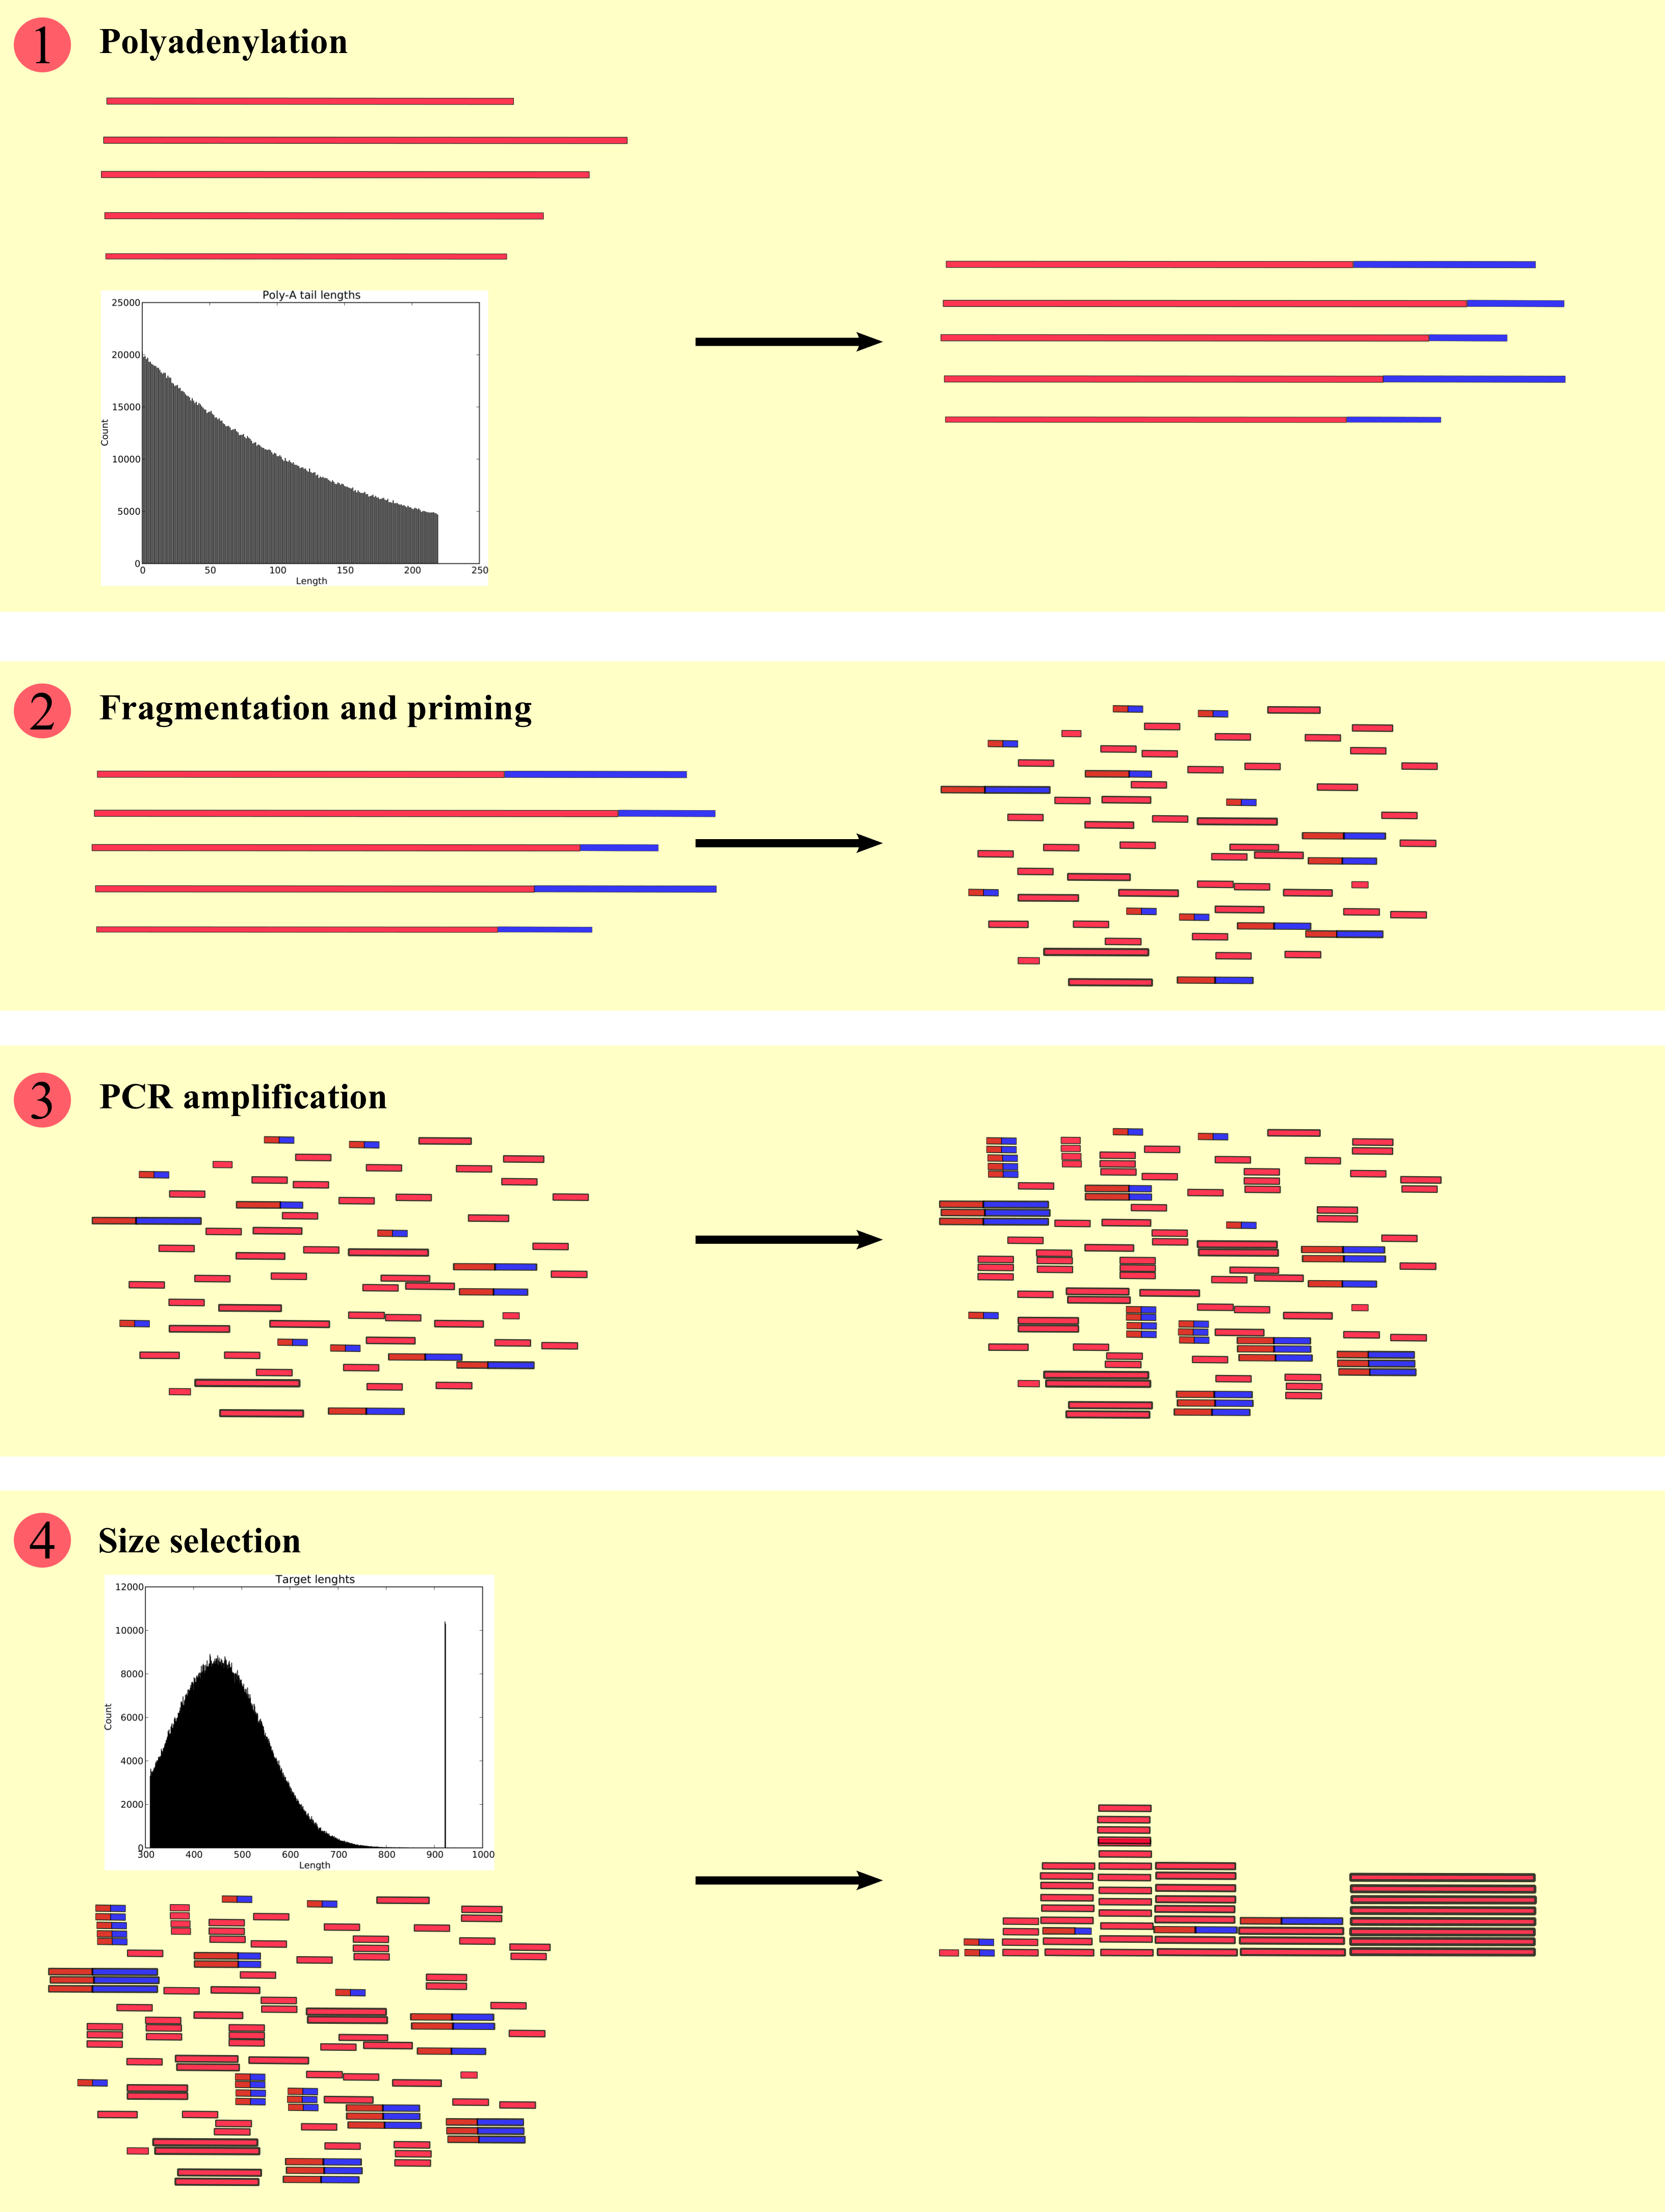
\includegraphics[scale=0.36]{pix/rlsim_main.png}
\end{center}

Notes:

\begin{itemize}
\item The fragment sampling (one of the most expensive steps) is performed in parallel using the concurrency capabilities of the {\tt Go} language. 
\item During RNA-seq library preparations, size selection is usually performed before PCR amplification. In \rlsim, for practical reasons, size selection is simulated after PCR amplification. In the majority of the cases this should not affect considerably the simulation of the interactions between size selection and other biasing factors.
\end{itemize}

\end{enumerate}

\subsubsection{Target size distributions}
\label{sss:target_mix}

The target length distributions used for the simulation of size selection and polyadenylation can be specified as mixture distributions with the syntax \emph{weight}:\emph{type}:\emph{parameters}. The available types are the following:

\begin{itemize}
\item{{\tt n} -- truncated {\bf normal} distribution \cite{dist_normal} parametrised as {\tt(}\emph{mean}, \emph{sd}, \emph{minimum}, \emph{maximum}{\tt )}. 
For example a truncated normal mixture component with mean 900, standard deviation 10 with minimum value 100 and maximum value 2000 can be specified as \texttt{n:(900, 10, 100, 2000)}}.
\item{{\tt sn} -- truncated {\bf skew normal} distribution \cite{dist_skew_normal} parametrised as \texttt{(}{\it location}, {\it scale}, {\it shape}, {\it minimum}, {\it maximum} \texttt{)}
A skew normal component with location 800, scale 50, shape 4 truncated between 600 and 1000 is specified as {\tt sn:(700,50,4,600,1000)}.}
\item{{\tt g} -- truncated {\bf gamma} distribution \cite{dist_gamma} parametrised as \texttt{(}\emph{mean}, \emph{shape}, \emph{minimum}, \emph{maximum}\texttt{)}. A gamma distribution with mean 600, shape 50, minimum value 400 and maximum value 1000 is specified as {\tt g:(600, 50, 400, 1000)}.
}
\end{itemize}

The mixture weight are normalised in order to sum to 1, hence an equal mixture of the example distributions above can be specified as:

\begin{verbatim}
1.0:n:(900, 10, 100, 2000) + 1.0:sn:(800,50,4,600,1000) + 1.0:g:(600,50, 400, 1000)
\end{verbatim}

, having a density similar to the one shown in the figure below:

\begin{center}
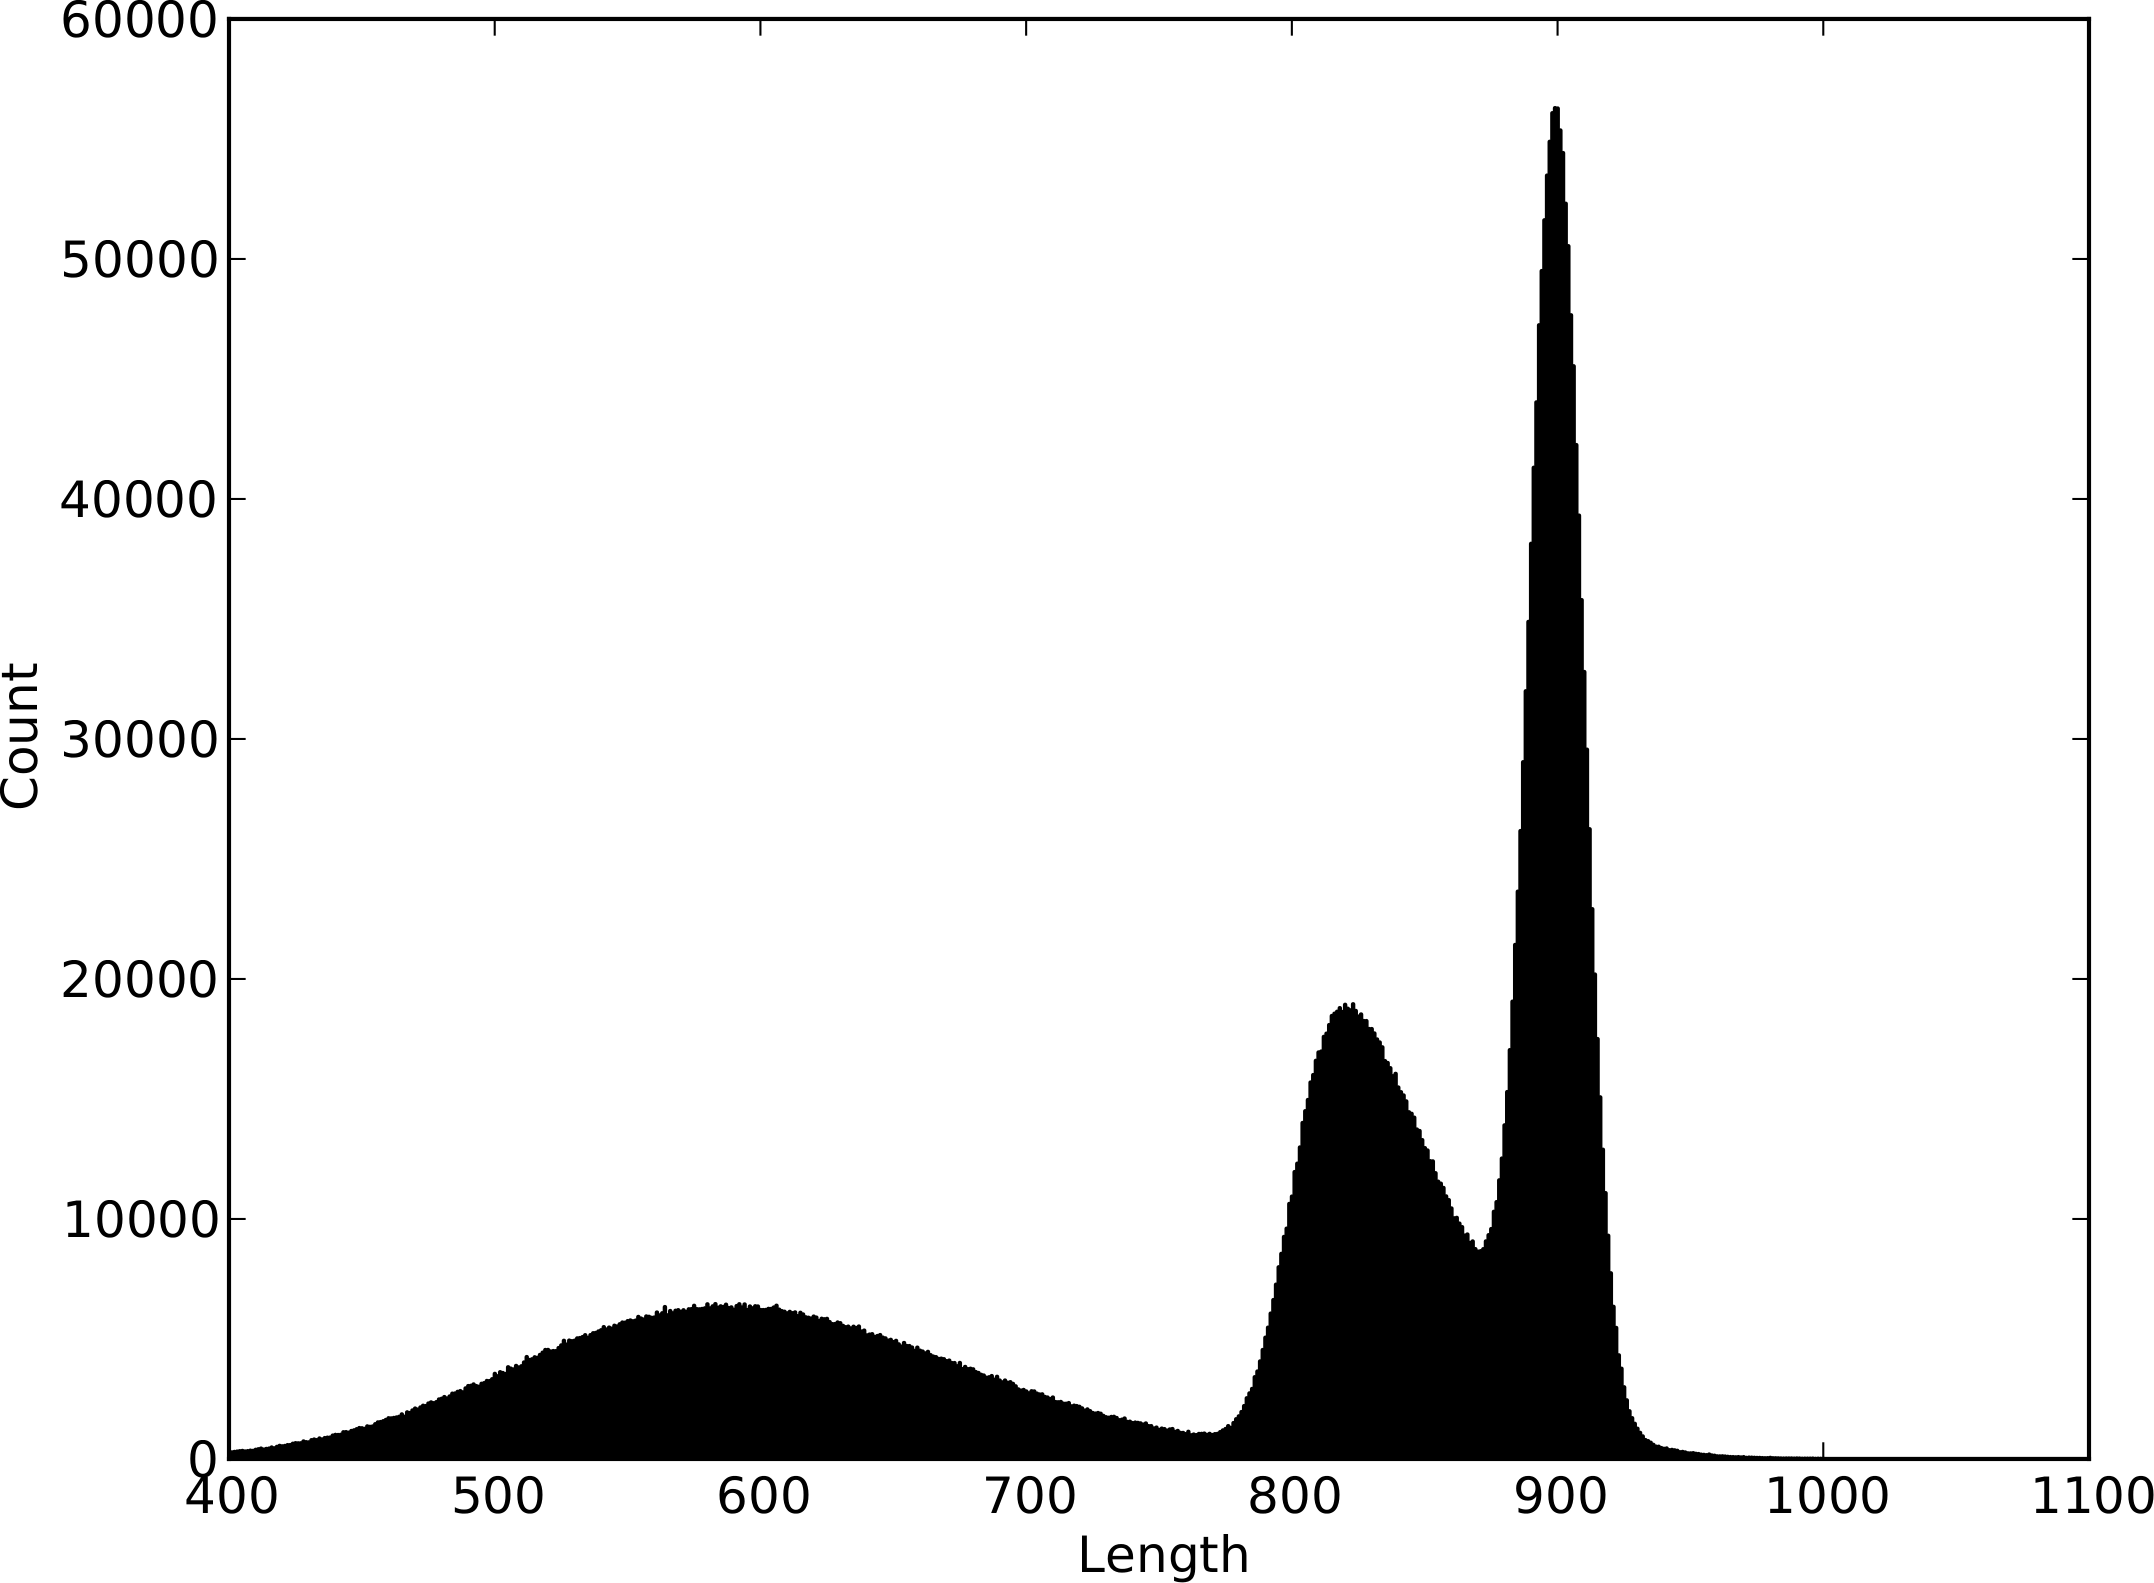
\includegraphics[scale=0.5]{pix/target_mix.png}
\end{center}

\subsubsection{Simulating polyadenylation}
\label{sss:polya_sim}

The target distribution of poly(A) tail lengths is specified as a mixture of truncated distributions via the {\tt -a} flag using the syntax described in section \ref{sss:target_mix}. Polyadenylation is simulated in the following steps:

\begin{itemize}
    \item During the processing of the input, the poly(A) tail with the maximum size (as inferred from the target distribution) is appended to the sequence of each transcript. 
    \item During the fragmentation of a given molecule, a length is sampled from the target distribution and the poly(A) tail is shortened to that length.
\end{itemize}

The simulation of polyadenylation is illustrated in the figure below:

\begin{center}
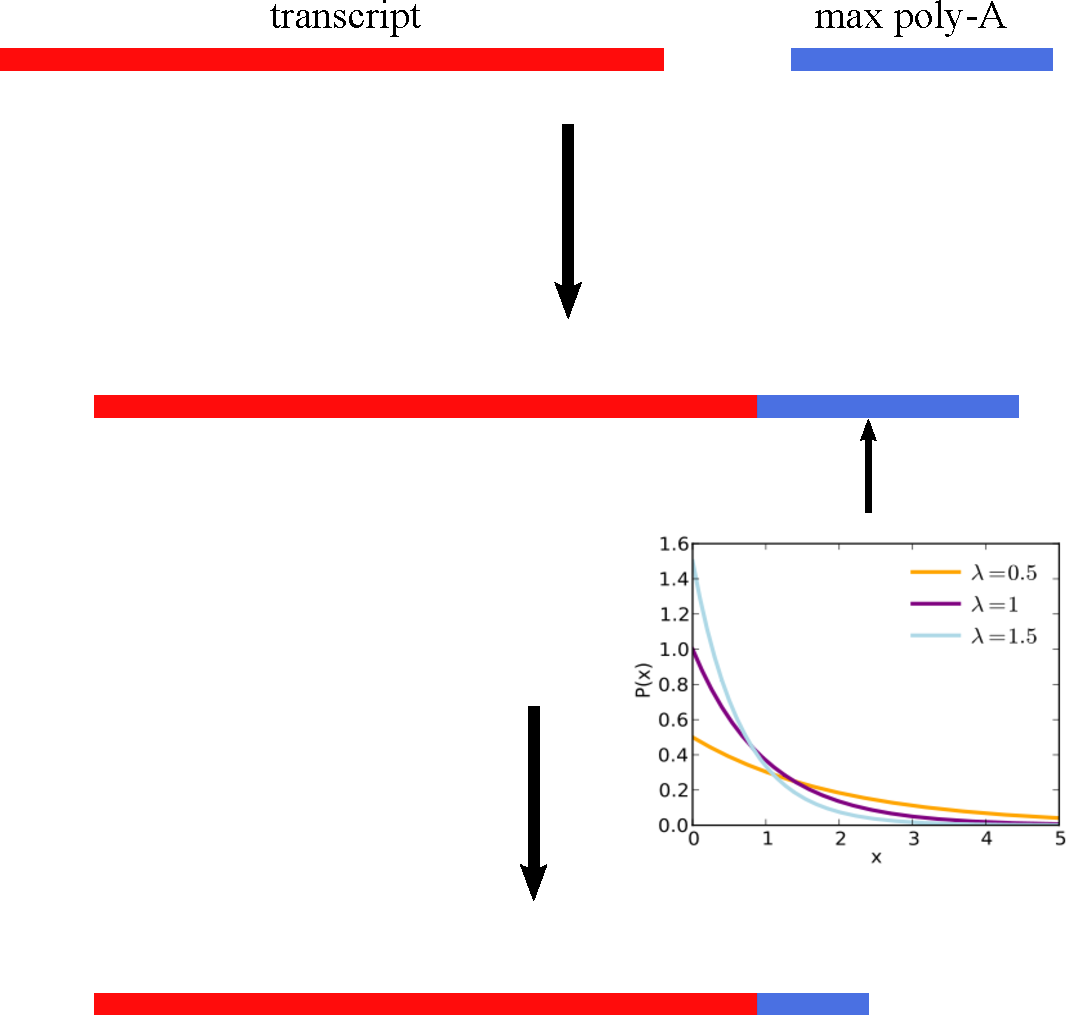
\includegraphics[scale=0.6]{pix/polya_simulation.pdf}
\end{center}

\subsubsection{A note on simulating TSS and poly(A) site variability}
\label{sss:tss_pa_varsim}

\rlsim uses the transcriptome as input, hence it cannot simulate the variability of polyadenylation and transcription start sites.
During the simulation it is assumed that the transcription starts at the first base of the transcript sequence and that the poly(A) tail is appended after
the last one. However, the user can still simulate these factors by simply including the TSS and poly(A) variants in the input fasta file as distinct transcripts.

\subsubsection{Simulating priming}
\label{sss:priming_sim}

Some of the fragmentation methods simulate priming based on the ``binding affinity'' of the first \texttt{-k} bases (6 by default) of the proposed fragment. The priming site is sampled using the following approach:

\begin{itemize}
    \item{Pre-calculate and cache the binding affinity of all sites in the transcript. 
    The first step in calculating the binding affinity is to calculate the change in free energy $\Delta G$ corresponding to the binding of the oligomer beginning with the respective base, based on a nearest-neighbor thermodynamic model \cite{santalucia04} with the ``temperature'' equal to the priming bias parameter $p$ (set by the \texttt{-p} flag). Then the binding affinity $K$ is calculated as:
\begin{equation}
    K = e^{-\frac{\Delta G}{Rp}}   
\end{equation}

, where $R$ is the universal gas constant.
    \item{During the simulation of fragmentation, the priming site within individual fragments is sampled proportionally to the pre-calculated binding affinities. The sampled priming site will define the new start or end position of the fragment.}
    }

\warn{The above approach for simulating priming bias is inspired by the physical model of oligonucleotide binding, but it ignores many important factors and so it is not a valid physical model itself! For example, it assumes that every fragment is primed once and only once, furthermore it ignores the effect of the concentrations of random oligomers. Hence, $p$ is a mere ``priming bias parameter'' and not real temperature on the Kelvin scale. Despite these caveats, we think that this approach is still useful for creating complex priming biases which are qualitatively similar to the ones observed in real data.}

Under positive priming bias parameters ($p$), the approach above will create a preference for G and C nucleotides, especially at the first and last bases of the oligomer. Negative priming parameters invert this, creating preference towards A and T nucleotides.

\end{itemize}

\subsubsection{Fragmentation methods}
\label{sss:frag_methods}

\rlsim has multiple fragmentation methods, some of them are inspired by actual protocols:

\begin{itemize}
\item {\tt after\_prim\_double -- \red{default}}
\item {\tt after\_noprim\_double}
\item {\tt pre\_prim}
\item {\tt after\_prim} 
\item {\tt after\_noprim}
\item {\tt pre\_prim}
\item {\tt prim\_jump}
\end{itemize}

The fragmentation methods are specified via the \texttt{-f} flag and optionally they can take a parameter separated with a ``\texttt{:}'' from the name of the approach (e.g. \texttt{"pre\_prim:2000"}).

In the section below we will briefly describe the fragmentation methods, their parameters and the characteristics of the data simulated using them. In order to illustrate the different fragmentation/priming methods, we will simulate data under two rather artificial settings in order to emphasize their effects on the sequence biases around the edges of the fragment and the sequence dependent coverage trends across the transcript.

\begin{enumerate}
        \item{The goal of the first simulation setting is to illustrate the \textbf{sequence specific biases} around the fragment edges. In order to clearly demonstrate these effects, we simulated fragments from a rather unrealistic random transcriptome composed of 500 transcripts of length 1000000 having uniform base composition and an expression level of 100. The length of the transcripts ensures that the effect of the fragmentation biases is minimised. The large number of random bases in the transcriptome ensures that most of the oligomers are represented in the input in an equal frequency. The other relevant parameters were the following:
        \begin{itemize}
            \item{The number of sampled fragments (\texttt{-n}): 5000000}
            \item{The target insert size distribution was a truncated normal with a mean of 200 and a standard deviation of 20: \texttt{"1.0:n:(200, 20, 150, 100000)"}}
            \item{The priming bias parameter (\texttt{-p}) was set to 5.0.} 
            \item{The length of the simulated poly(A) tail (\texttt{-a}) was set to 1, unless indicated otherwise.}
            \item{In most simulations the simulation of PCR amplification was disabled by setting the number of cycles to 0.}
            \item{In the cases where PCR amplification was simulated, we used 11 cycles with the following GC efficiency parameters: \texttt{"(0.2, 0.5, 0.95)"}}
            \item{Sequencing was simulated using \texttt{simNGS}, with the read length set to 75.}
            \item{The simulated reads were aligned back to the transcriptome using \texttt{BWA} in paired-end mode.}
            \item{The sequence bias plots were produced using the \texttt{pb\_plot} tool.}
        \end{itemize}

        The simulation pipeline and the raw output can be found under the \texttt{src/test/pos\_bias} directory in the \rlsim repository.
        }
        \item{
        The second simulation setting illustrates how the sequence specific and fragmentation biases manifest themselves as \textbf{uneven coverage across the the transcripts}. In order to illustrate this, we simulated from a transcript with a total length of 3500, composed of alternating GC rich and AT rich units of length 35, having an expression level of 400000. Other relevant simulation parameters:
        \begin{itemize}
            \item The number of requested fragments (\texttt{-n}) was 40000.
            \item{The target insert size distribution (\texttt{-d}) was a truncated normal with a mean of 200 and a standard deviation of 20: \texttt{"1.0:n:(200, 20, 150, 20000)"}}
            \item{The priming bias parameter (\texttt{-p}) was set to 1.0, producing very strong sequence biases.} 
            \item{The strand bias parameter (\texttt{-b}) was set to 0.0, corresponding to generating a ``stranded'' library.}
            \item The length of the simulated poly(A) tail (\texttt{-a}) was set to 1.
            \item{In most simulations the simulation of PCR amplification was disabled by setting the number of cycles to 0.}
            \item{In the cases where PCR amplification was simulated, we used 30 cycles with the following GC efficiency parameters: \texttt{"(8.0,0.2,0.95)"}}
            \item{Sequencing was simulated using \texttt{simNGS}, with the read length set to 50.}
            \item{The simulated reads were aligned back to the transcript using \texttt{BWA} in paired-end mode.}
            \item{The sequence bias plots were produced using the \texttt{plot\_cov} tool, which plots the \emph{base coverage} of individual reference bases using the colors blue for A and T, and red for G and C.}
        \end{itemize}

        The simulation pipeline and the raw output can be found under the \texttt{src/test/cov} directory in the \rlsim repository.
        }
\end{enumerate}

\warn{Please note that the simulations above were deliberately designed to emphasize the effects of different fragmentation/priming methods. When simulating from real transcriptomes and more reasonable parameters these effects will combine in a complex manner, making them less apparent and harder to link them to specific features in the coverage.}

Given the lack of sufficient of knowledge about the RNA fragmentation process \emph{in general}, the fragmentation methods implemented in \rlsim do not apply sophisticated approaches for the RNA fragmentation itself, but they try to produce a fragment pool with a length distribution similar to the specified target distribution. This is generally done by trying to match the average fragment lengths produced by fragmentation to the mean lengths of the mixture components.  

\paragraph{{Fragmentation method: }\texttt{after\_prim\_double}}

This is the default fragmentation method, inspired by the standard, non-stranded Illumina RNA-seq protocol.
It is meant to introduce sequence specific ``priming'' biases near the start and end of the fragment.
Fragmentation is simulated on the level of individual transcript ``molecules'', meaning that if a transcript has an expression level of 100, than fragmentation will be simulated a hundred times, each fragment produced during these simulation is registered in a ``fragment pool'' which later is subject to PCR simulation and size selection.

The fragmentation of a single transcript is done in following steps, as illustrated in the figure below:
\begin{enumerate}
    \item{As a first step, a mixture component is sampled from the target mixture specified by the user.}
    \item{The number of breakpoints is sampled from a Poisson distribution such that the average length of produced fragments will be equal to \emph{twice} the mean of the mixture component sampled in the first step. The reason for doubling the average fragment length is to compensate for the shortening effects of the priming simulation performed later on. Alternatively the mean fragment length can be specified as a parameter passed to the fragmentation method (e.g. \texttt{"after\_prim\_double:600"})}
    \item{The breakpoints are sampled \emph{uniformly} across the length of the transcript. The beginning of the transcript and the end of the poly(A) serve as pre-defined ``extra'' breakpoints.}
    \item{All the fragments which are outside of the range of the specified target mixture are discarded right away.}
    \item{Priming is simulated on the forward and reverse strands as described in section \ref{sss:priming_sim} in order to select a new fragment start and end.}
    \item{The fragment is discarded with a probability set by the \texttt{-flg} flag, which allows for the tuning of the total number of fragments produced from a fixed input transcriptome.}
    \item{Finally, the fragment is registered in the fragment pool which later is subject to PCR simulation and size selection.}
\end{enumerate}

%ch f after_prim double
\begin{center}
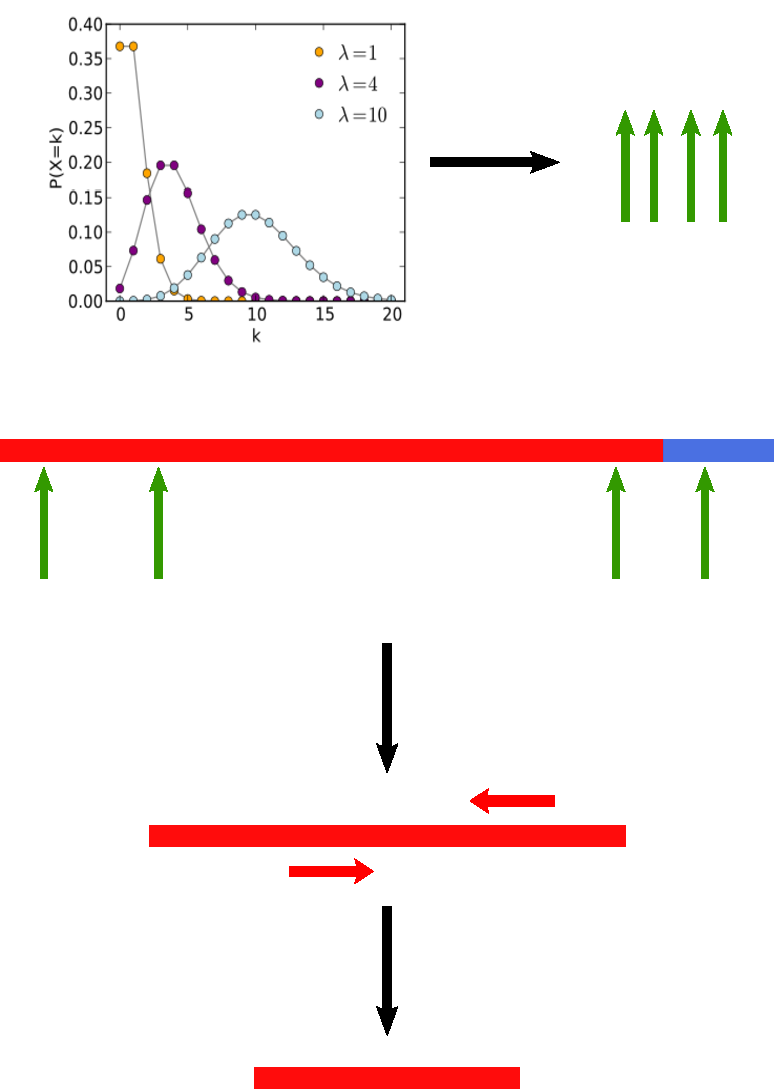
\includegraphics[scale=0.6]{pix/after_prim_double.pdf}
\end{center}

From the output of the first simulation setting using \texttt{after\_prim\_double} it is apparent that this method introduces
sequence specific biases both near the the fragment start and end. The priming simulation prefers G and C nucleotides leading to higher
binding affinities, especially at the first and last bases of the oligomer: 

\begin{center}
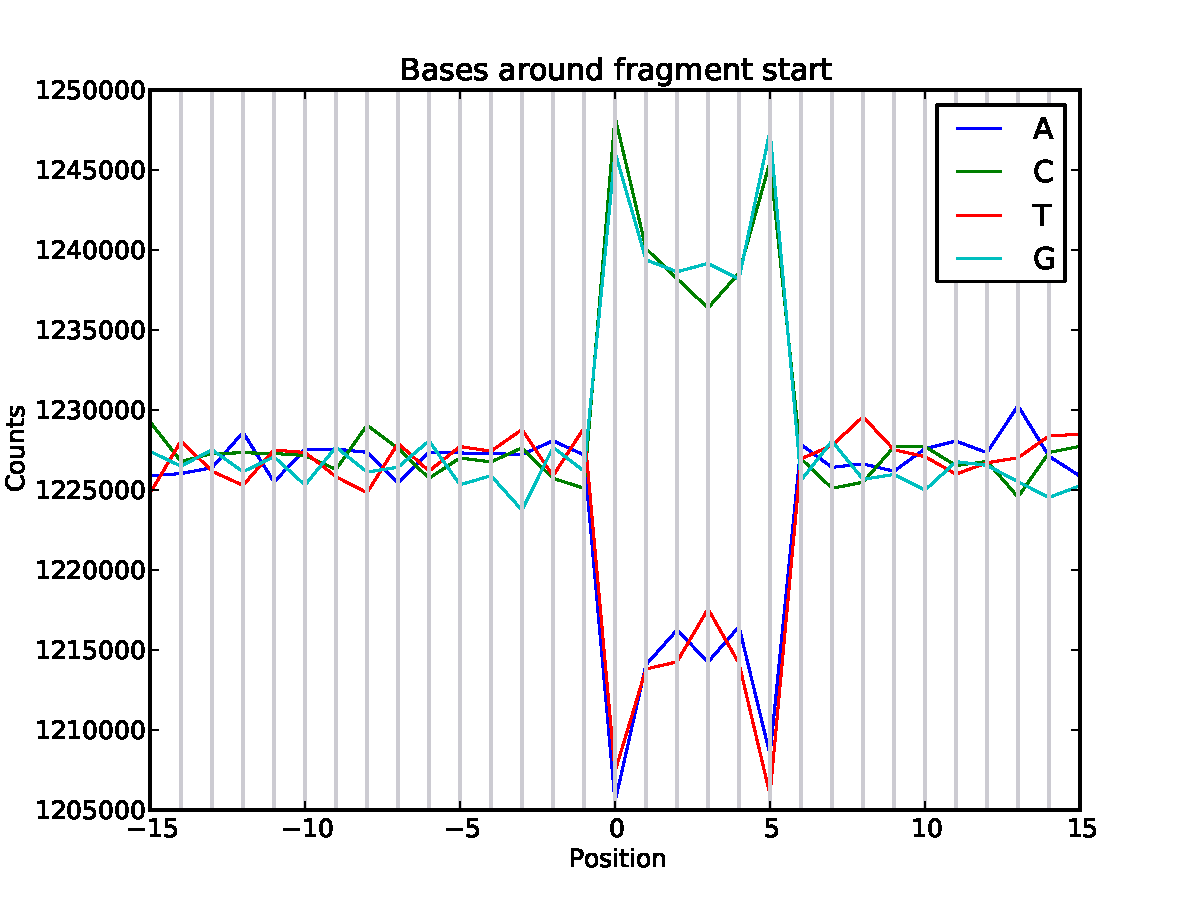
\includegraphics[scale=0.6,page=1]{../src/test/pos_bias/pb_after_prim_double.pdf}
\\
\includegraphics[scale=0.6,page=2]{../src/test/pos_bias/pb_after_prim_double.pdf}
\end{center}

The preference towards G and C nucleotides is also manifested as an unequal coverage across the example transcript in the second simulation,
leading to higher base coverage in GC-rich regions:

\begin{center}
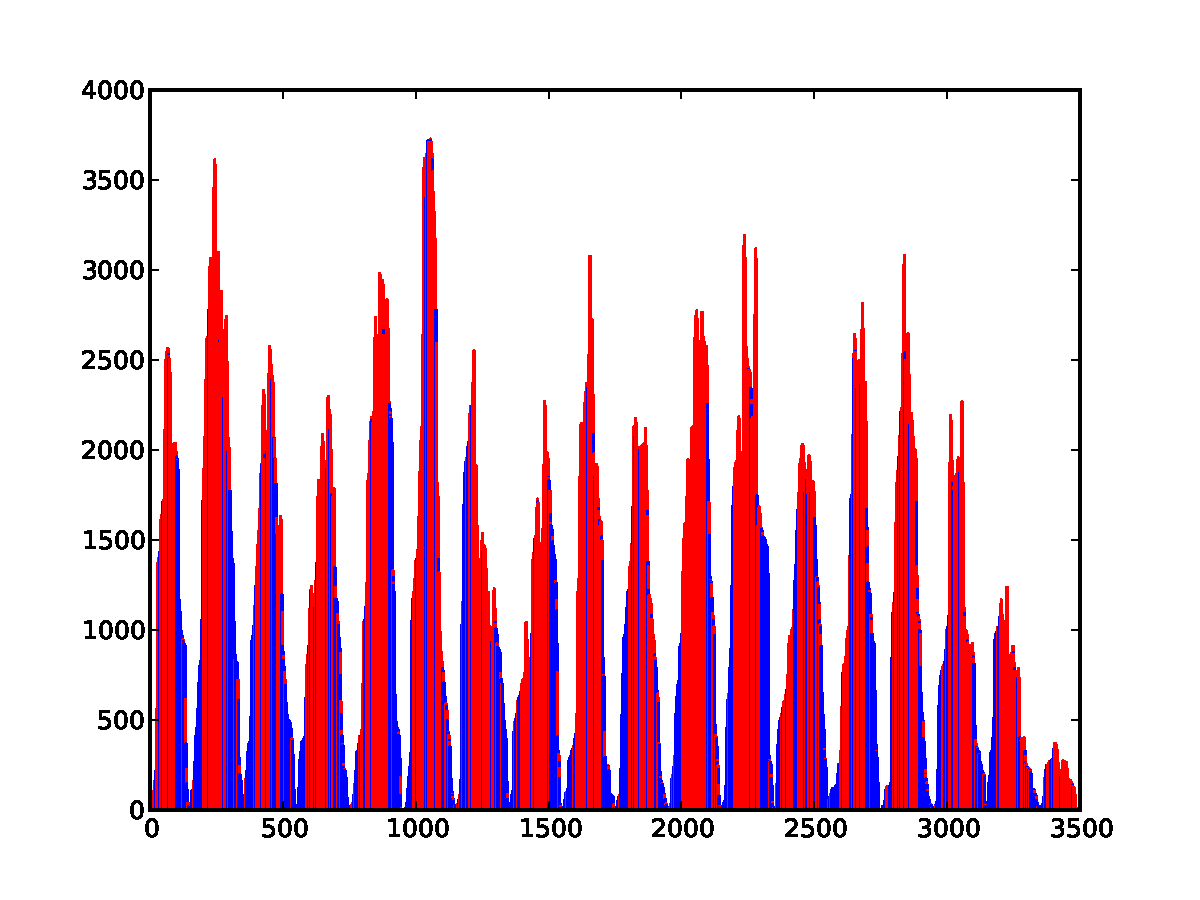
\includegraphics[scale=0.6,page=1]{../src/test/cov/cov_after_prim_double.pdf}
\end{center}


\paragraph{{Fragmentation method: }\texttt{after\_noprim\_double}}
% after_noprim_double

This fragmentation method is very similar to the \texttt{after\_prim\_double} method described above, with one important difference: the priming sites are sampled uniformly, without making use of the binding affinities. Hence this method produces a fragment pool similar to the previous method, but without introducing sequence specific biases. This is apparent from the output of the first simulation setting, showing an essentially random distribution of nucleotides around fragment start and end:

\begin{center}
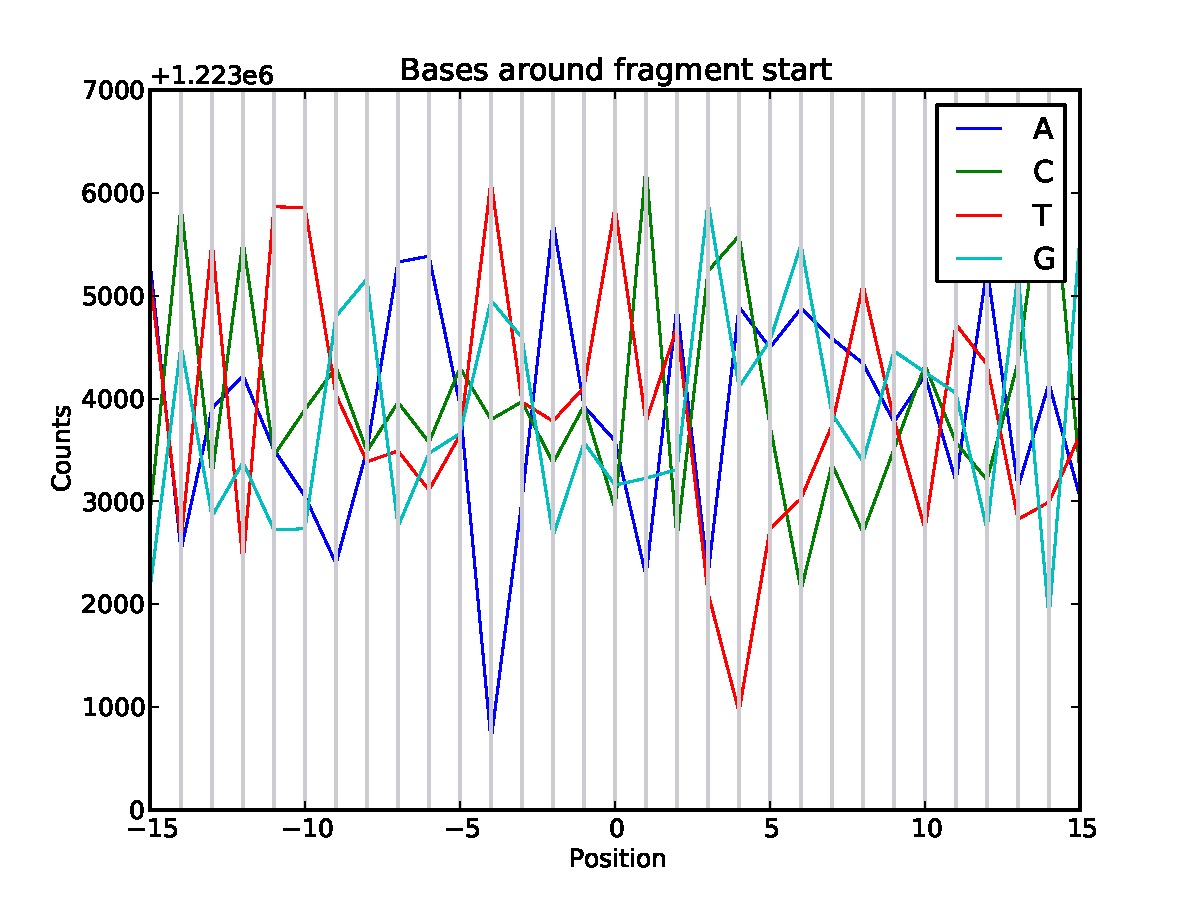
\includegraphics[scale=0.6,page=1]{../src/test/pos_bias/pb_after_noprim_double.pdf}
\\
\includegraphics[scale=0.6,page=2]{../src/test/pos_bias/pb_after_noprim_double.pdf}
\end{center}

Also, the output of the second simulation setting shows how the base coverage is no longer correlated with the GC content, however we can still observe the
characteristic coverage biases around the 3' and 5' of the transcript due to fragmentation, size selection and strandedness:

\begin{center}
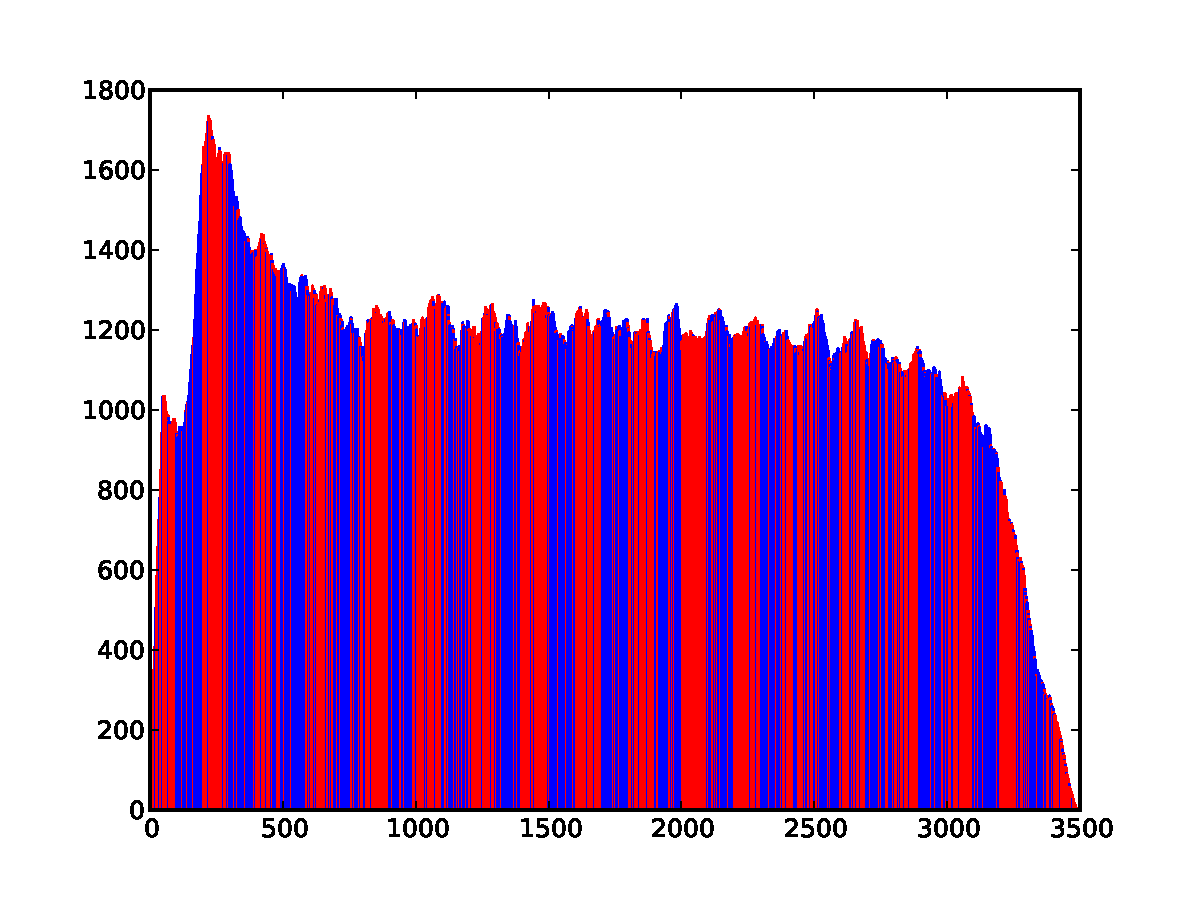
\includegraphics[scale=0.6,page=1]{../src/test/cov/cov_after_noprim_double.pdf}
\end{center}


\paragraph{{Fragmentation method: }\texttt{after\_prim}}
% after_prim

This fragmentation method is similar to \texttt{after\_prim\_double}, however the binding affinities are used only when sampling the start of the fragment.

\begin{center}
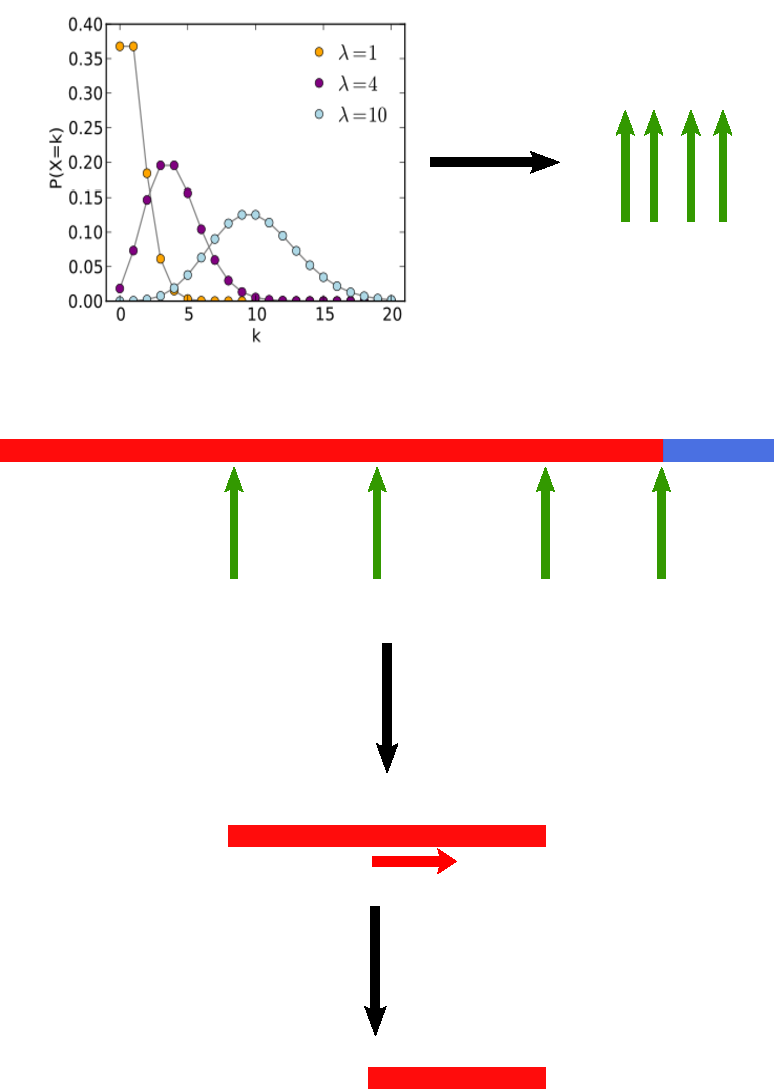
\includegraphics[scale=0.6]{pix/after_prim.pdf}
\end{center}

This leads to a sequence specific bias near the start of the fragment, but a random distribution of nucleotides around the end:

\begin{center}
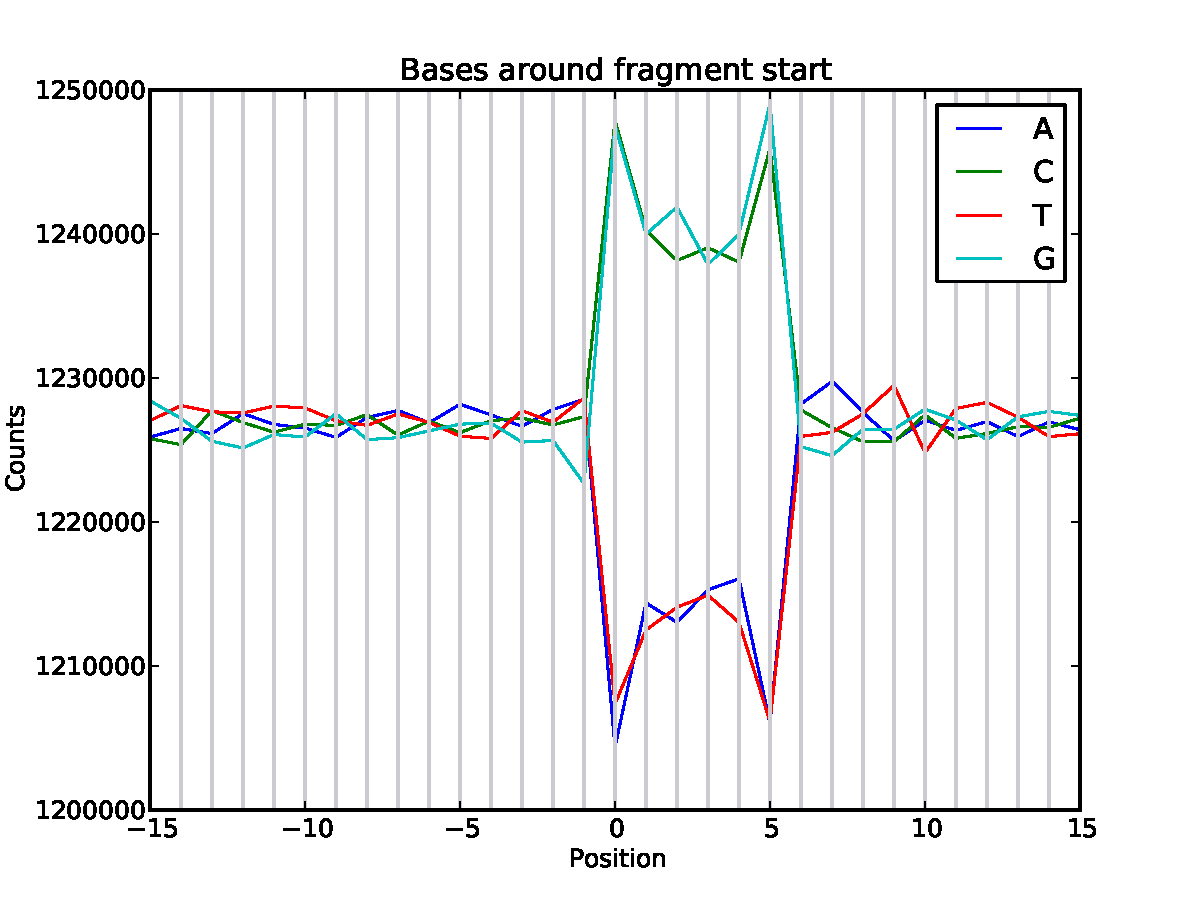
\includegraphics[scale=0.6,page=1]{../src/test/pos_bias/pb_after_prim.pdf}
\\
\includegraphics[scale=0.6,page=2]{../src/test/pos_bias/pb_after_prim.pdf}
\end{center}

This method, similarly to \texttt{after\_prim\_double} increases coverage in GC rich regions:

\begin{center}
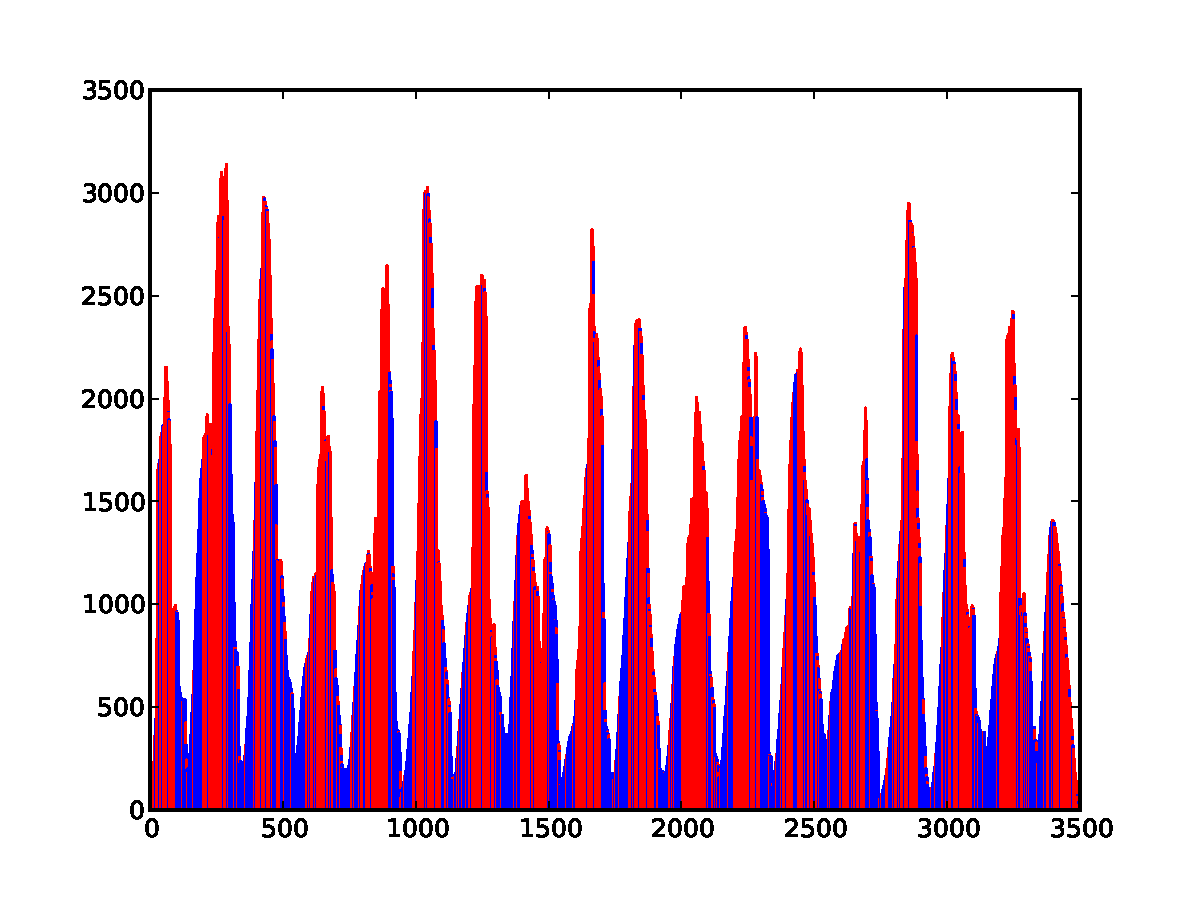
\includegraphics[scale=0.6,page=1]{../src/test/cov/cov_after_prim.pdf}
\end{center}


\paragraph{{Fragmentation method: }\texttt{after\_noprim}}
% after_noprim

This fragmentation method is a modification of \texttt{after\_prim}, with uniformly sampled priming sites.
It produces no sequence specific biases near fragment start and end:

\begin{center}
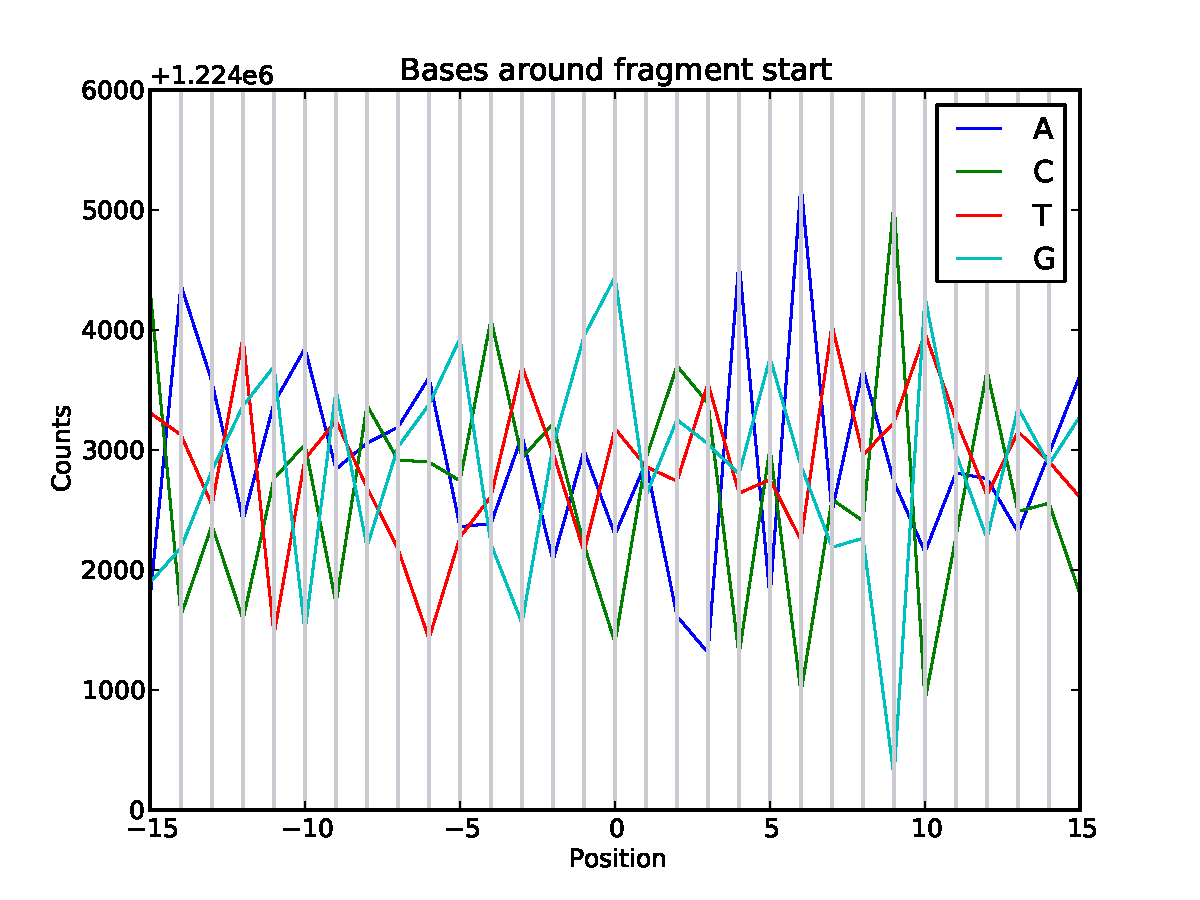
\includegraphics[scale=0.6,page=1]{../src/test/pos_bias/pb_after_noprim.pdf}
\\
\includegraphics[scale=0.6,page=2]{../src/test/pos_bias/pb_after_noprim.pdf}
\end{center}

The coverage trends due to fragmentation, size selection and strandedness are still apparent:

\begin{center}
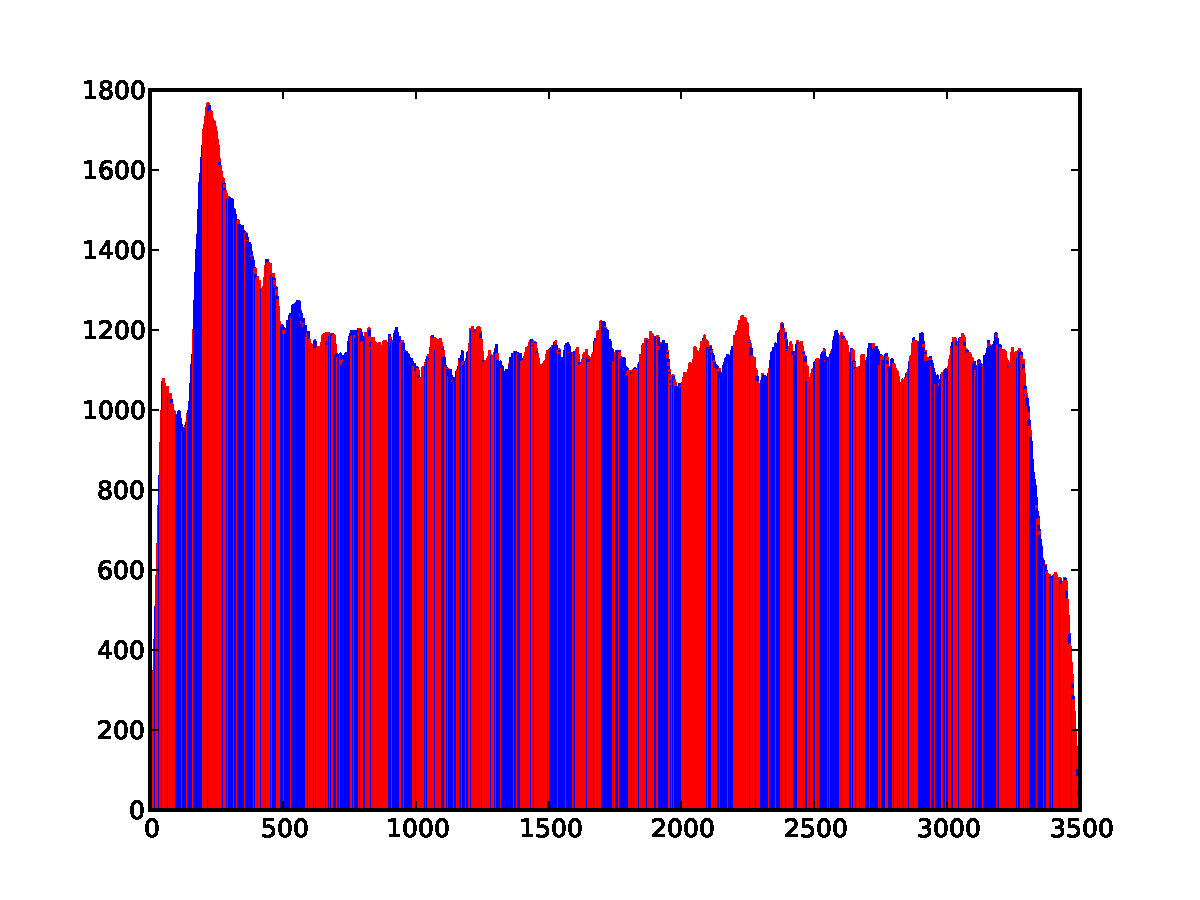
\includegraphics[scale=0.6,page=1]{../src/test/cov/cov_after_noprim.pdf}
\end{center}

\paragraph{{Fragmentation method: }\texttt{pre\_prim}}
% pre_prim

This fragmentation method is inspired by the RNA-seq protocols which perform reverse transcription primed in the poly(A) tail.
The fragmentation consists of the following steps:

\begin{enumerate}
    \item{The method does \emph{not} simulate the ``sliding'' of the poly-T primer over the poly(A) tail but it assumes that priming always happens right at the end. However, the subsequent fragmentation step introduces similar effects to ``primer sliding''.}
    \item{Elongation is simulated by sampling the cDNA length from a geometric distribution with a mean specified by the mandatory parameter taken by the fragmentation method (e.g. \texttt{"pre\_prim:1500"}). The sampled elongation length defines the new start of the transcript.}
    \item{Breakpoints are sampled similarly to the \texttt{after\_noprim\_double} method, without doubling the average length of the produced fragments.}
    \item{Fragments with lengths outside the target mixture are discarded.}
    \item{Fragment loss is simulated according to the probability specified by the \texttt{-flg} flag.}
    \item{The remaining fragments are registered in the fragment pool.}
\end{enumerate}

\begin{center}
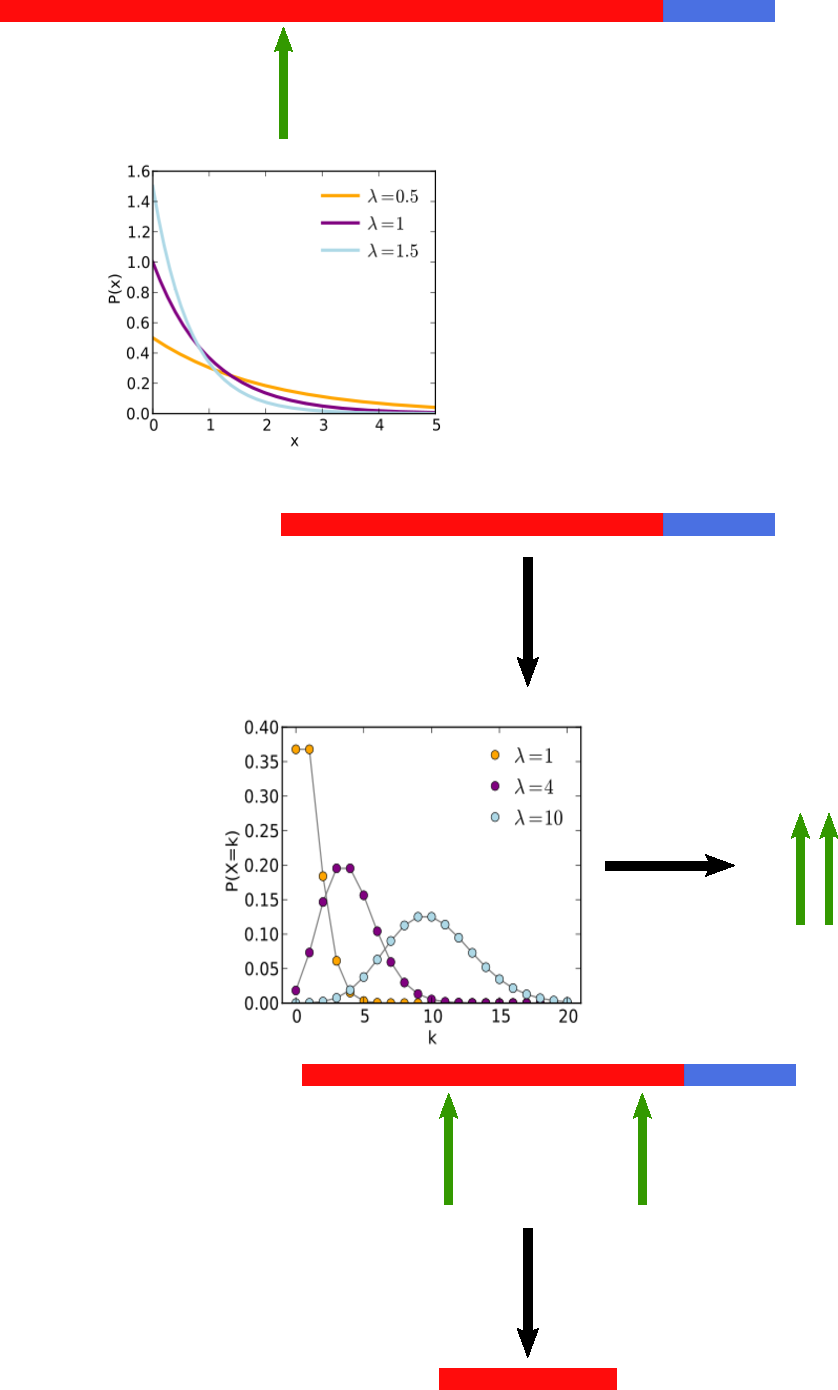
\includegraphics[scale=0.6]{pix/pre_prim.pdf}
\end{center}

This fragmentation method does not introduce sequence specific biases in an explicit manner, as it is apparent from the output of the first simulation:

\begin{center}
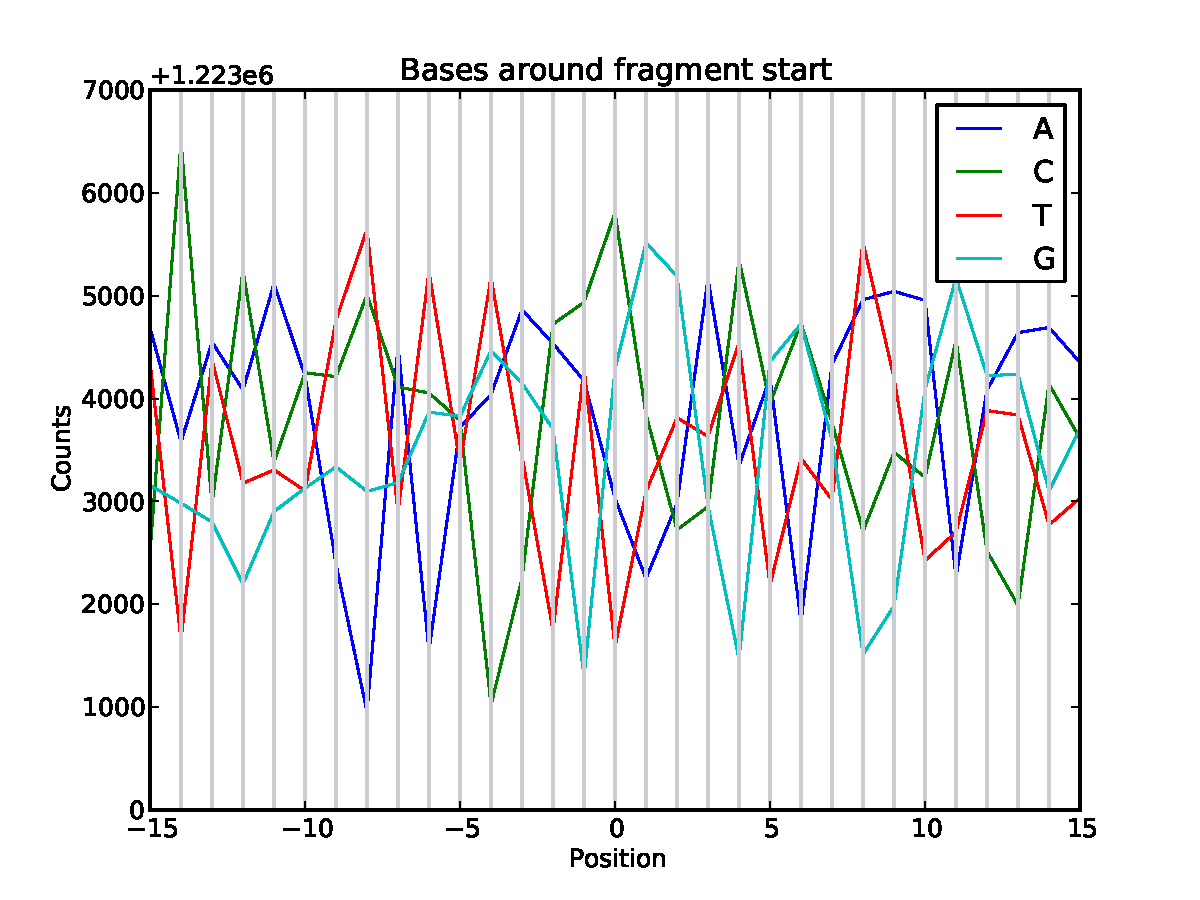
\includegraphics[scale=0.6,page=1]{../src/test/pos_bias/pb_pre_prim.pdf}
\\
\includegraphics[scale=0.6,page=2]{../src/test/pos_bias/pb_pre_prim.pdf}
\end{center}

This method explicitly introduces a coverage bias towards the 5' end of the transcript, the strength of which depends on the specified mean elongation length
parameter:

\begin{center}
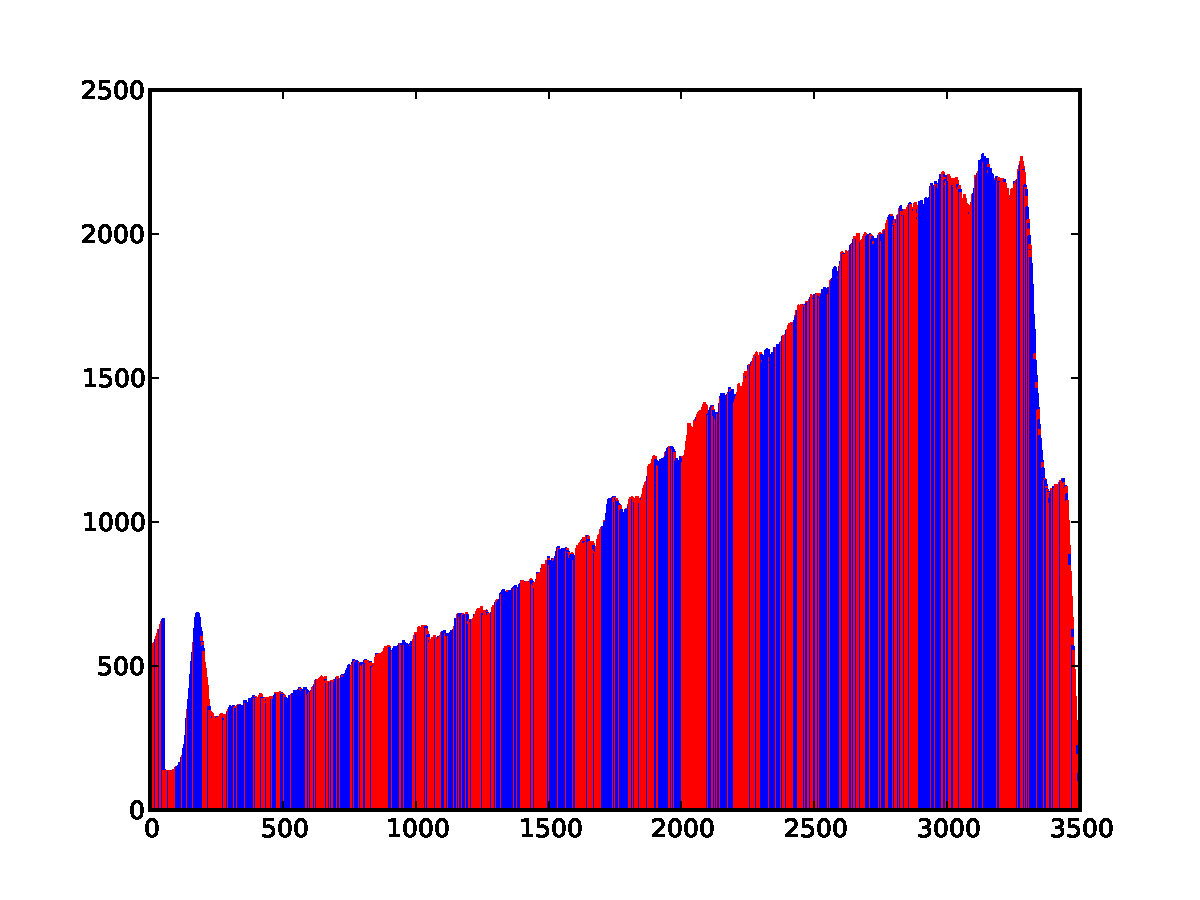
\includegraphics[scale=0.6,page=1]{../src/test/cov/cov_pre_prim.pdf}
\end{center}

\warn{This fragmentation method takes the mean elongation length as a mandatory parameter. It is important to carefully choose this parameter as with the default value the simulation might not produce the desired output.}

\paragraph{{Fragmentation method: }\texttt{prim\_jump}}
% prim_jump

This fragmentation method has no biological inspiration, however it is able to introduce both sequence specific biases and 5' coverage biases in a complex manner, providing an opportunity to stress-test advanced bias correction methods.
The following steps are performed:

\begin{enumerate}
    \item{The start of the fragment is sampled by simulating priming across the whole length of the transcript.}
    \item{The end of the fragment is defined by sampling the fragment length from the target length distribution.}
    \item{After simulation of loss, the fragment is registered in the fragment pool.}
    \item{The steps above are iterated over the remaining portion of the transcript until the end of the poly(A) tail is reached.}
\end{enumerate}

\begin{center}
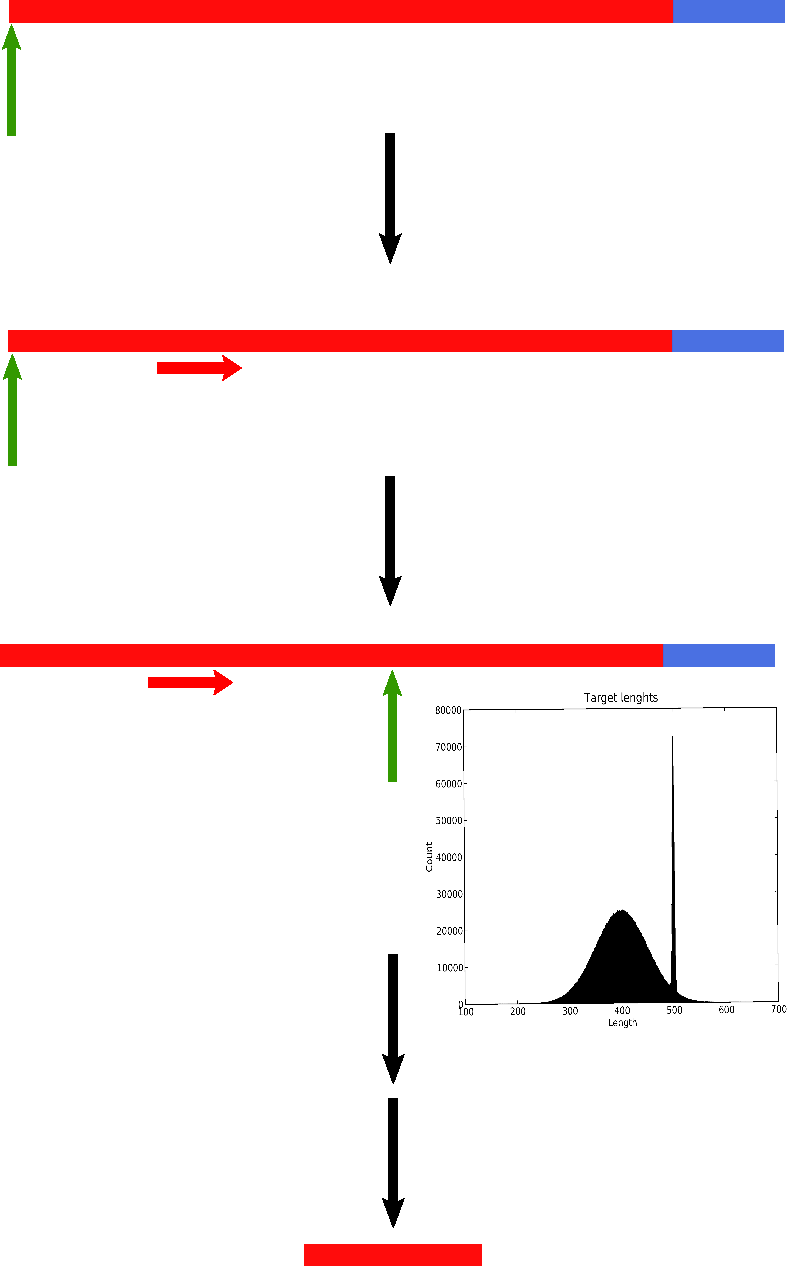
\includegraphics[scale=0.6]{pix/prim_jump.pdf}
\end{center}

This method introduces sequence specific biases near the start, but not the end of the fragment:

\begin{center}
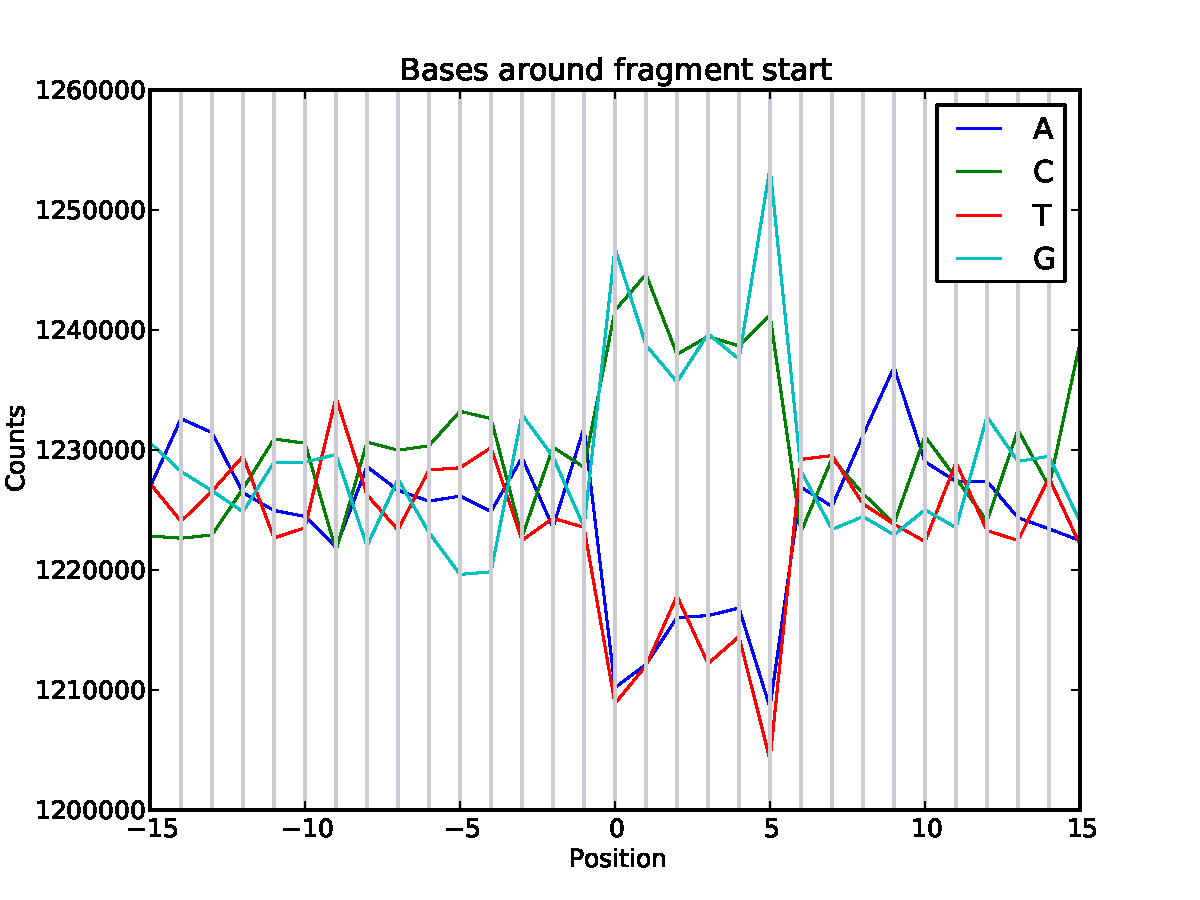
\includegraphics[scale=0.6,page=1]{../src/test/pos_bias/pb_prim_jump.pdf}
\\
\includegraphics[scale=0.6,page=2]{../src/test/pos_bias/pb_prim_jump.pdf}
\end{center}

Besides the preference towards CG rich regions, it also introduces a coverage bias towards the 5' end of the transcript,
as demonstrated by the output of the second simulation setting:

\begin{center}
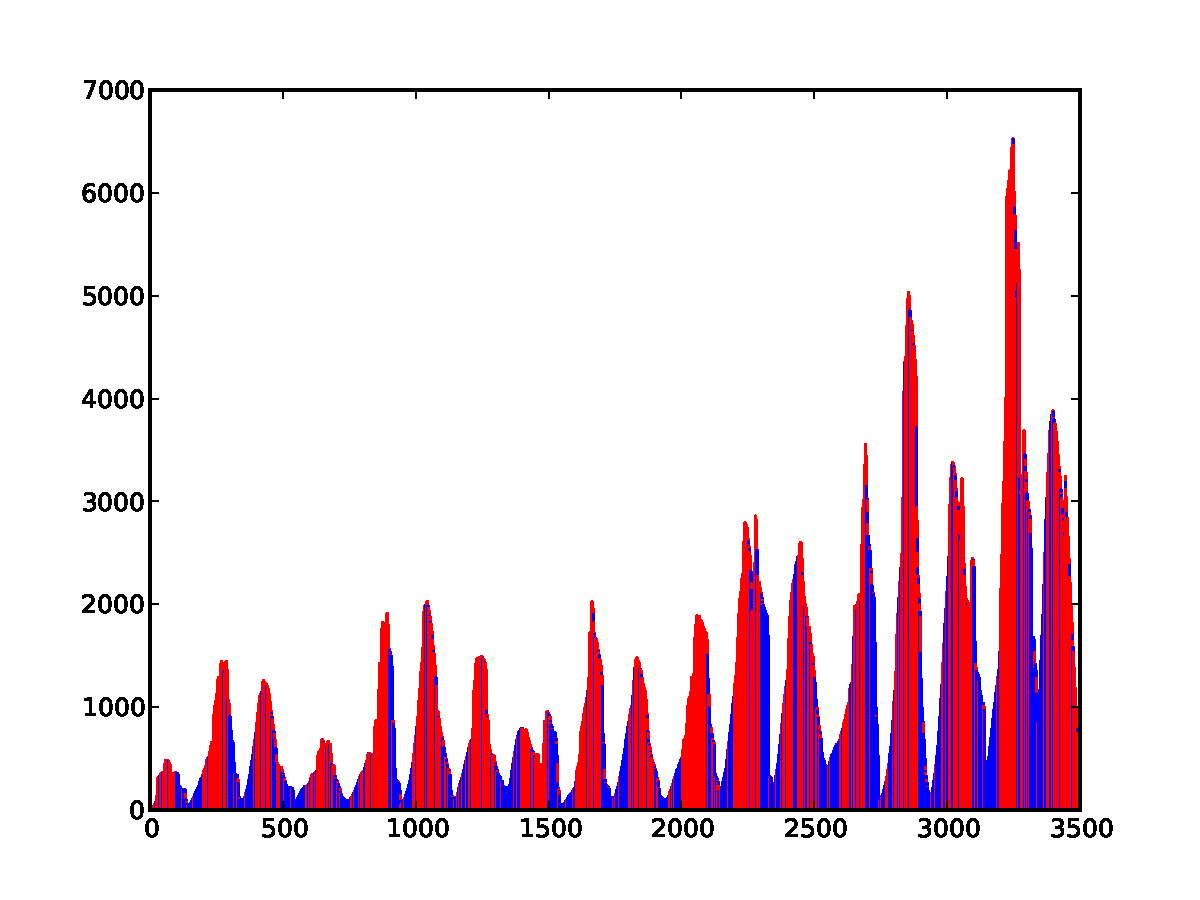
\includegraphics[scale=0.6,page=1]{../src/test/cov/cov_prim_jump.pdf}
\end{center}


\subsubsection{Simulating PCR amplification}

A central concept in the \rlsim PCR simulation framework is the ``amplification efficiency''\footnote{\warn{The term ``efficiency'' (denoted as $\epsilon$) is used through this document as the probability of replication, in contrast with the quantitative PCR literature, in which efficiency usually means the expected number of descendants of a single molecule after a single cycle (equal to $1 + \epsilon$).}}, which is the probability that 
a fragment is replicated during a cycle. In the \rlsim framework the amplification efficiency can be fragment specific (as described below), but it is always constant throughout the cycles.

The PCR simulation takes the fragment pool generated by the fragmentation process (containing fragments with initial count $C_0$) and outputs a fragment pool
with amplified fragment counts.
If $C_i$ is the count for a given fragment and $\epsilon$ is the amplification efficiency, the amplified count after one cycle ($C_{i+1}$) is calculated as:

\begin{equation}
    C_{i+1} = C_i + Binomial(n=c_i, p=\epsilon)
\end{equation}

This step is repeated until the number of PCR cycles is equal to the value of the \texttt{-c} flag.

Amplification efficiencies can be specified in many ways:

\begin{itemize}
    \item{\textbf{Fixed amplification efficiency}: if the \texttt{-e} flag is set, its value will be used as a amplification efficiency \emph{for all fragments}, regardless of length and GC content.}
    \item{Alternatively the GC dependent efficiency can be set through the \texttt{-eg} flag and the length efficiency through the {-el}. The actual amplification efficiency is calculated as the product of the GC and length efficiencies.}
    \item{The ``raw parameter'' JSON files generated by \effest and provided by the \texttt{-j} flag superseeds the \texttt{-eg} flag, and so \rlsim will use the respective empirical GC efficiencies. A minimum GC efficiency can be specified through the \texttt{-jm} flag.}
\end{itemize}

\vspace{1em}\textbf{Specifying GC dependent efficiencies}\vspace{1em}

The \texttt{-eg} flag accepts strings formatted as \texttt{"(${\alpha}$, $m$, $M$)"}, where $m$ is the minimum efficiency, $M$ is the maximum efficiency and $\alpha$ is a shape parameter. Then the amplification efficiency of a fragment with GC content $g_i$ is calculated as:

\begin{equation}\label{eq:gc_eff}
    \epsilon_{g_i} = m + (M-m) \left(1 - g_i^\alpha\right)^\alpha
\end{equation}

For example \texttt{"(8.0,0.5,0.95)"} defines the following mapping between GC content and amplification efficiency:

\begin{center}
    \includegraphics[type=pdf,ext=.json.pdf,read=.json.pdf,scale=0.6,page=2]{../src/test/basic/rlsim_report}
\end{center}

\warn{The \texttt{-eg} flag provides an easy way to specify GC dependent efficiencies, but it can be too restrictive. The user can specify however an arbitrary discrete GC efficiency function by tweaking a ``raw parameter'' file generated by the \effest tool.}

\vspace{1em}\textbf{Specifying length dependent efficiencies}\vspace{1em}

The length dependent efficiencies are specified through the \texttt{-el} flag as a string formatted as \texttt{"($\beta$, $m$, $M$)"}, where $m$ and $M$ are the minimum and maximum efficiencies and $\beta$ is a shape parameter. The efficiencies are calculated as:

\begin{equation}
    \epsilon_{l_i} = l_{i}^{-\beta}
\end{equation}

, and then scaled in order to have the minimum $m$ and maximum $M$ over the range of the target size distribution specified via the \texttt{-d} flag.

For example, if the target size distribution is \texttt{"1:n:(300,20,100,5000)"} and the length efficiency parameter is \texttt{"(0.4,0.5,1.0)"}, the mapping between lengths and efficiencies is:

\begin{center}
    \includegraphics[type=pdf,ext=.json.pdf,read=.json.pdf,scale=0.6,page=3]{../src/test/basic/rlsim_report}
\end{center}

\warn{Note than the length dependent efficiencies are set to 1.0 by default.}

\vspace{1em}\textbf{Calculating the joint efficiency function}\vspace{1em}

The ``joint efficiency function'' determining the amplification efficiency of a fragment with a given GC content and length is then
calculated as the product of the two components:

\begin{equation}
    \epsilon = \epsilon_{g_i} \times \epsilon_{l_i}
\end{equation}

For example, the GC and length components above lead to the following joint efficiency mapping:

\begin{center}
    \includegraphics[type=pdf,ext=.json.pdf,read=.json.pdf,scale=0.6,page=12]{../src/test/basic/rlsim_report}
\end{center}

The simulated PCR amplification will create a preference towards fragments with certain GC contents.
For example the first simulation setting uses a GC efficiency function preferring fragments with low GC content, which manifests in the output
as a sequence specific bias over the whole length of the fragment:

\begin{center}
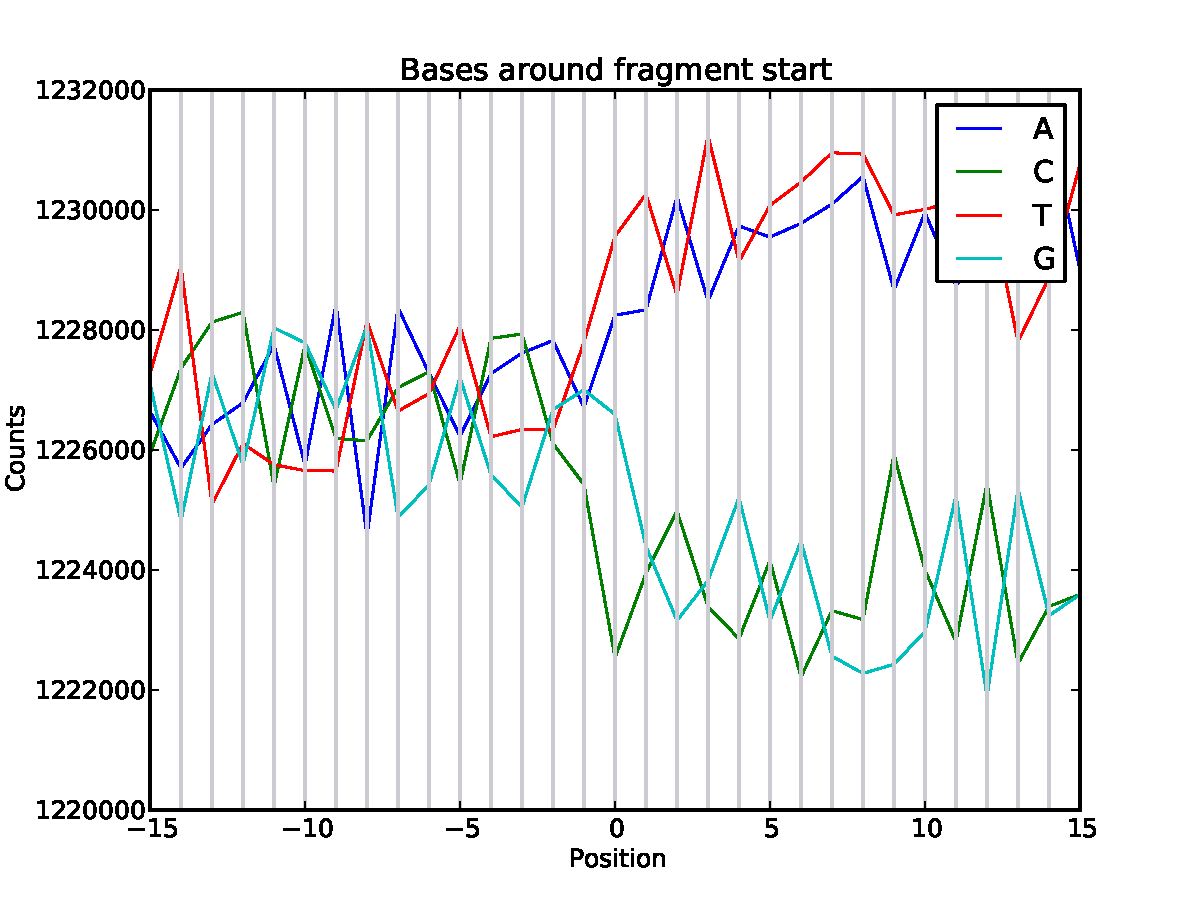
\includegraphics[scale=0.6,page=1]{../src/test/pos_bias/pb_pcr.pdf}
\\
\includegraphics[scale=0.6,page=2]{../src/test/pos_bias/pb_pcr.pdf}
\end{center}

The preference for regions with low GC content can be spotted in the base coverage trends in the output of the second simulation setting as well.
Note how simulated PCR alone can create complex trends in base coverage:

\begin{center}
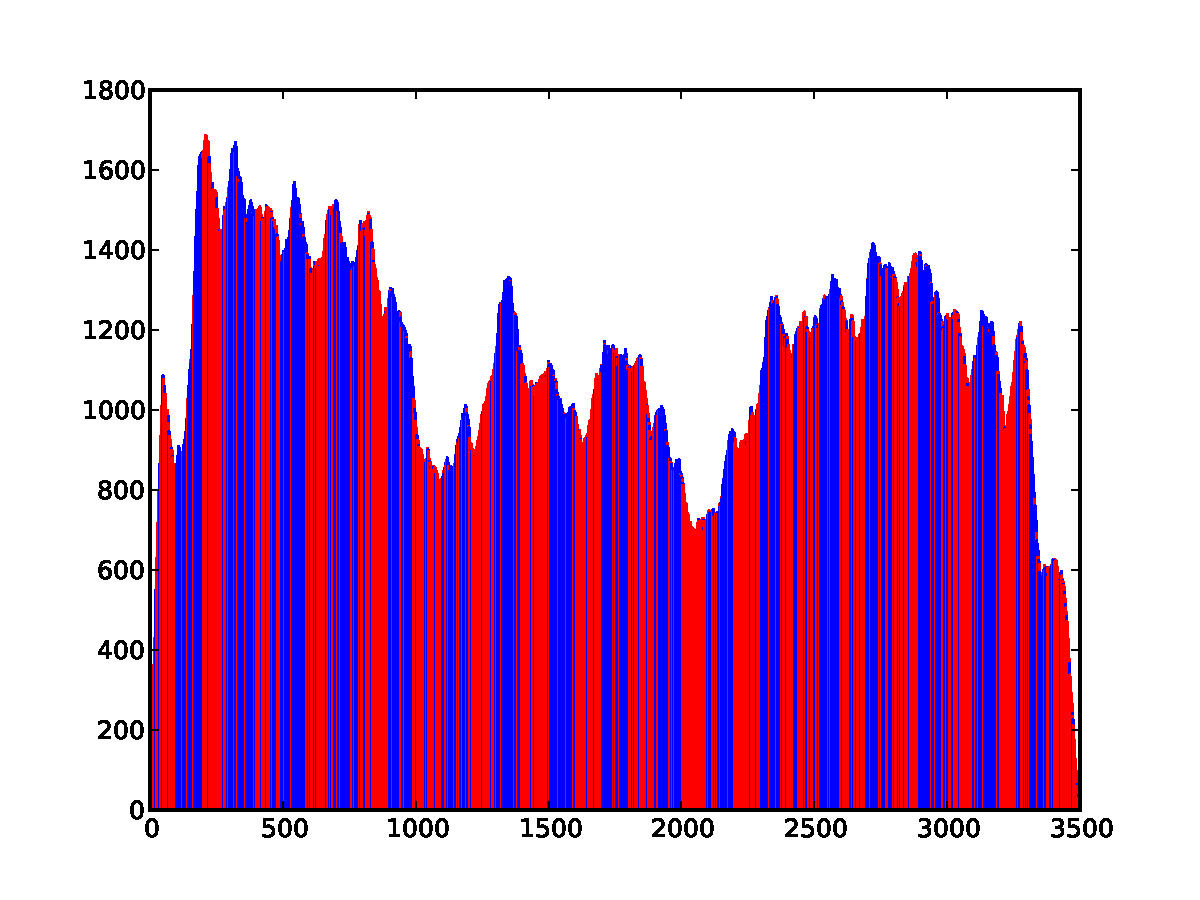
\includegraphics[scale=0.6,page=1]{../src/test/cov/cov_pcr.pdf}
\end{center}

\subsubsection{Interactions of simulated biases}

Biases due to the fragmentation process, priming and PCR simulation can interact in a complex way. In most cases the output of such simulations will require interpretation by statistical approaches. However, in the idealised case of the first simulation setting we can enable both priming and PCR simulation and observe how these factors combine in order to create a more complex sequence specific bias:

\begin{center}
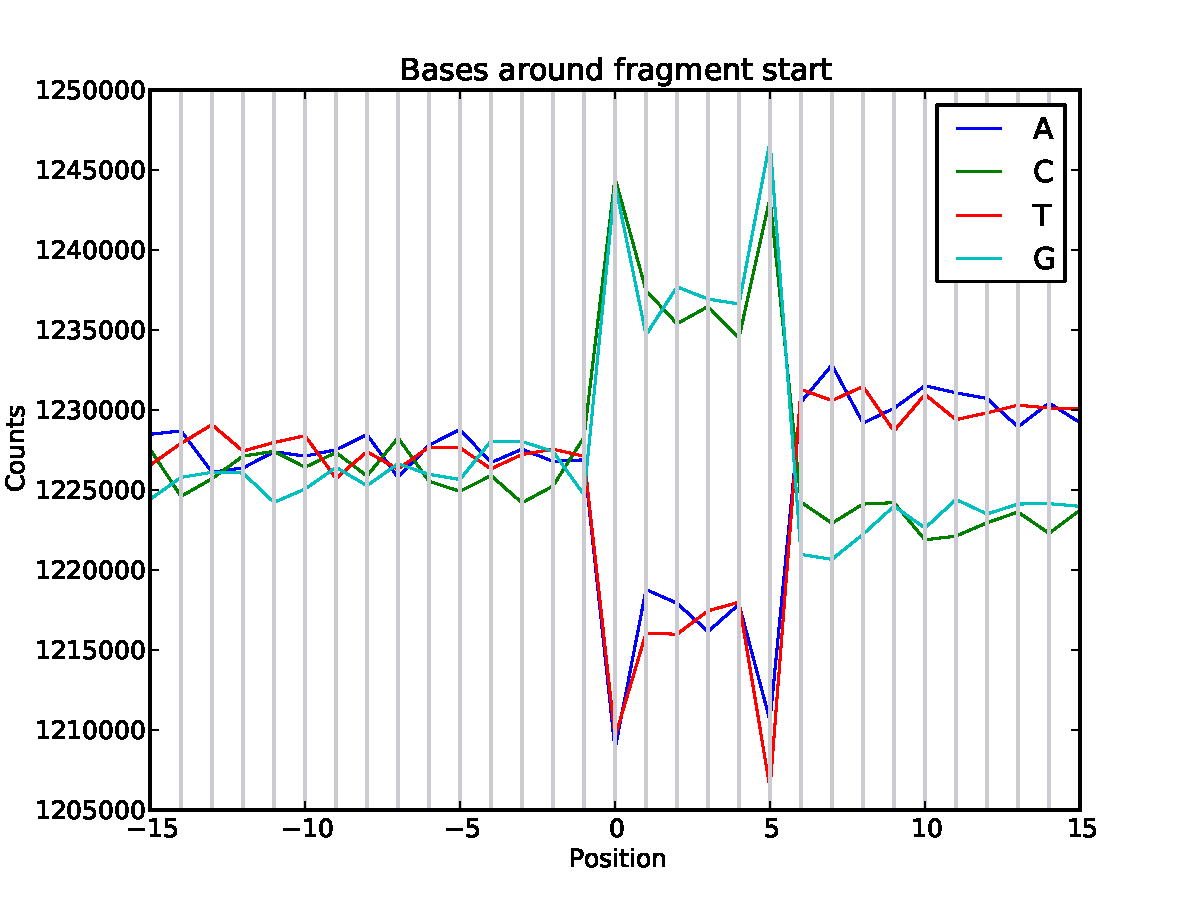
\includegraphics[scale=0.6,page=1]{../src/test/pos_bias/pb_full.pdf}
\\
\includegraphics[scale=0.6,page=2]{../src/test/pos_bias/pb_full.pdf}
\end{center}

In the simulation settings above the simulation of polyadenylation was practically disabled by setting the tail length to 1.
Now if besides the priming and PCR simulation we also simulate longer tails with a mean length of 200, we can also observe how this leads to a slight increase
in the frequency of A nucleotides after the sixth base of the fragment:

\begin{center}
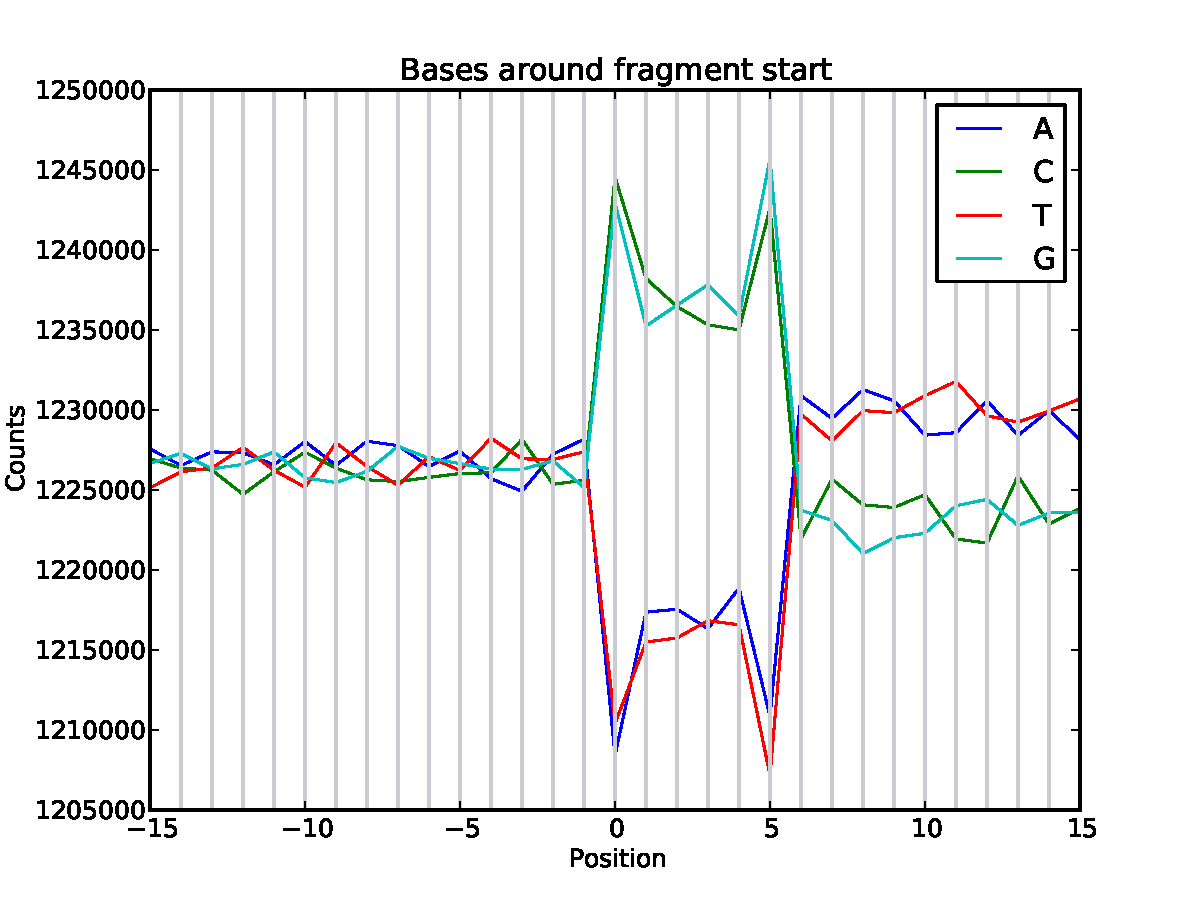
\includegraphics[scale=0.6,page=1]{../src/test/pos_bias/pb_full_polya.pdf}
\\
\includegraphics[scale=0.6,page=2]{../src/test/pos_bias/pb_full_polya.pdf}
\end{center}

This increase in A frequencies is likely to due to the spurious mappings of the A-rich reads coming from the poly(A) tails. This effect seems to have an impact regardless of the relatively long simulated read length (75 bases).

In the light of the relatively complex bias patterns produced by the simple simulations above it is clear how using more realistic parameters and real transcriptomes can produce convoluted biases which allow for the benchmarking of advanced bias correction methods.

\subsection{Running the program}

\begin{verbatim}
    Usage:
        rlsim [arguments] [transcriptome fasta files (optional)]
\end{verbatim}

\subsubsection{Input files}

The input files specified after the command line arguments are the transcriptome fasta files with the transcript expression levels
encoded in the sequence names using \texttt{\$} as separator. So a transcript named \texttt{trA} with expression level 100 has the following fasta record:

\begin{verbatim}
>trA$100
GCTTCCGGCATCTGGCTCAGTTCCGCCATGGCCTCCTTGGAAGTCAGTCGTAGTCCTCGCAGGTCTCGGCGGGAGCTG ...
...
\end{verbatim}

If no input files are specified, \rlsim will attempt to read the input transcriptome from the standard input.

\subsubsection{Command line arguments}

Command line arguments not detailed in the previous sections:

\begin{itemize}
    \item[\texttt{-n}]{The number of requested fragments (no default, required if no raw parameter file is specified).}
    \item[\texttt{-b}]{The probability of sampling the fragment from the forward strand (default: 0.5).}
    \item[\texttt{-c}]{The number of simulated PCR cycles (default: 11).}
    \item[\texttt{-flg}]{The probability of losing a fragment after fragmentation and before PCR simulation (default: 0.0).}
    \item[\texttt{-m}]{Multiplier to increase the expression level of all transcripts and so decrease the sampling ratio (default: 1.0).}
    \item[\texttt{-r}]{The name of the report JSON file (default: \texttt{rlsim\_report.json}).}
    \item[\texttt{-t}]{The maximum number of cores to use. It is used to set the \texttt{runtime.GOMAXPROCS} variable, also limits the number of gorutines spawned (default: 4).}
    \item[\texttt{-g}]{Keep the fragments in memory instead of using a disk cache. This speeds up the simulation, but it is only usable if the input transcriptome is small or if there is sufficient memory available (default: false).}
    \item[\texttt{-si}]{Initial random seed (default: set from UTC time).}
    \item[\texttt{-sp}]{Random seed used for PCR amplification and sampling (default: seeded from the initial RNG).}
    \item[\texttt{-ss}]{Random seed used for fragment sampling (default: seeded from the PCR RNG).}
    \item[\texttt{-v}]{Toggle verbose messages (default: false).}
    \item[\texttt{-h}]{Display help message and exit.}
    \item[\texttt{-V}]{Display version and exit.}
    \item[\texttt{-prof}]{Enable CPU profiling and write info to the specified file (default: "").}
    \item[\texttt{-gcfreq}]{Explicitly trigger garbage collection after this many transcripts (defaults: 100).}
    \item[\texttt{-rng}]{Generate test output for the random number generators (default: off).}
\end{itemize}

\subsubsection{Output}

\rlsim produced the following output:

\begin{itemize}
    \item{The simulated fragments are written out to the standard output in fasta format. The format of the name field is similar to the one used by the \texttt{simLibrary} tool: 
    \begin{center}
    {>Frag\_\textit{frag\_nr} \textit{transcript\_name} (Strand \textit{strand} Offset \textit{start} -- \textit{end})}
    \end{center}
    }
    \item{The \rlsim report file (named \texttt{rlsim\_report.json} by default) contains various information about the simulation in JSON format. 
    It is parsed by the \plotRlsim tool, transforming it into a PDF report.} 
\end{itemize}

If invoked with the \texttt{-v} flag, \rlsim outputs verbose messages about the ongoing simulations. 
Most of the messages are self-explanatory, but some of them are worth mentioning in detail:
\begin{itemize}
    \item{The ``\textbf{total number of fragments in the pool}'' is the number of fragments in the fragment pool after simulating PCR.}
    \item{The ``\textbf{sampling ratio}'' is the number of sampled fragments divided by the total number of fragments in the pool. This is important, as in many cases the interactions of the different biases can be modulated by this ratio. The sampling ratio under a fixed input transcriptome can be modified by setting the fragment loss probability through the \texttt{-flg} flag. Higher fragment loss probabilities lead to smaller fragment pools and so higher sampling ratios.}
    \item{In some cases the input transcriptome and the specified parameters produce a fragment pool which does not have enough fragments in some length categories requested by the user via the total number of fragments and the target size distribution. These are reported by \rlsim as ``\textbf{missing fragments}''.}
\end{itemize}

\subsubsection{Advanced examples}

\vspace{1em}\paragraph{Simulating PCR pseudo-replicates}

\rlsim allows the user to change the random seeds used at different points during simulation, which allows for the simulation
of pseudo-replicates of different kinds. For example, PCR pseudo-replicates are simulated in the following steps:

\begin{enumerate}
    \item{Run a simulation with the initial and PCR random seeds specified via the \texttt{-si} and \texttt{-sp} flags:
        \begin{verbatim}
$ ./rlsim -n 2000 -si 112 -sp 200 test/basic/test_transcripts.fas > frags_rep1.fas
        \end{verbatim}
    }
    \item{Run a second simulation with the same input and parameters and the same initial, but a \emph{different PCR random seed}:
        \begin{verbatim}
$ ./rlsim -n 2000 -si 112 -sp 300 test/basic/test_transcripts.fas > frags_rep2.fas
        \end{verbatim}
    }
\end{enumerate}

Using the same input and initial random seed ensures that the composition of the fragment pools after fragmentation is exactly same in the two simulations.
The random seed specified through the \texttt{-sp} flag will initialise a new random number generator used throughout PCR simulation and fragment sampling. By specifying different seeds we can simulate distinct PCR amplifications of the same fragment pool and the subsequent sampling of fragments. This allows for assessing the effects of variation introduced by the respective processes.

\warn{Note, that for the different PCR pseudo-replicates the input fragment pool is exactly the same. In real experiments this pool is split into sub-pools which serve as templates for the PCR replicates. For practical reasons, \rlsim does not simulate this splitting process (for that we call the output ``pseudo-replicates''), however this is probably is safe to ignore in most of the cases.}

\vspace{1em}\paragraph{Simulating sampling pseudo-replicates}

A sampling pseudo-replicate is equivalent to technical replicates performed by sequencing the output of a given library many times.
Again, the \rlsim replicates are not proper replicates, as in contrary to real experiments they are performed \emph{with replacement}. However, if the sampling ratio is sufficiently small, again, this can be safely ignored.

The sampling pseudo-replicates are simulated as following:

\begin{enumerate}
    \item{Run a simulation with the initial and sampling random seeds specified via the \texttt{-si} and \texttt{-sp} flags:
        \begin{verbatim}
$ ./rlsim -n 2000 -si 212 -ss 400 test/basic/test_transcripts.fas > frags_rep1.fas
        \end{verbatim}
    }
    \item{Run a second simulation with the same input and parameters and the same initial, but a \emph{different sampling random seed}:
        \begin{verbatim}
$ ./rlsim -n 2000 -si 212 -ss 600 test/basic/test_transcripts.fas > frags_rep2.fas
        \end{verbatim}
    }
\end{enumerate}

The output of the two simulations are fragments sampled from the same fragment pool.

